\documentclass[10pt,a4paper]{amsart}
\usepackage{amsmath,amssymb,amsthm,graphicx}
\usepackage{amsmath,amssymb,graphicx,xcolor,mathtools,stmaryrd}
\providecommand{\coloneq}{\coloneqq}
\title{Soundness of usable-rule and argument-filtered reduction-pair processors for innermost constrained rewriting}
\author{Carsten Fuhs, Liye Guo, Cynthia Kop}
\date{doi:10.4230/LIPIcs.FSCD.2025.20; CC BY4.0}
\begin{document}
\maketitle
\noindent\textit{Editorial note.} Source https://drops.dagstuhl.de/entities/document/10.4230/LIPIcs.FSCD.2025.20. © Carsten Fuhs, Liye Guo and Cynthia Kop, CC BY4.0. Official HTML transcription with full author proof appendix and original diagrams retained.\par\medskip
\noindent\textit{Allowed standard prerequisites (editorial).}\begin{itemize}
\item Reducibility-candidate computability for accessible function-passing higher-order rewriting. Author §2 and Theorem6 (reference13) give the RC-set construction; standard computability closure facts are named in AppendixA2. All new innermost-chain and processor proof obligations are retained.
\end{itemize}\medskip
% BEGIN S2
 
\par\medskip\noindent\textbf{2 Preliminaries}\par
 
% BEGIN S2.p1
 
This section collects the preliminaries from the literature. First, we recall the definition of an LCSTRS [22].111In contrast to [22] and following [21], we assume that $\ell$ is a pattern in every rewrite rule ${\ell}\rightarrow{r}\ [\varphi]$. For notational convenience, we also assume that $\operatorname{Var}(r)\setminus\operatorname{Var}(\ell)\subseteq\operatorname{Var}(\varphi)$, which can be guaranteed by a simple transformation and is also adopted in the second half of [22]. Then, we recollect from [13] the definition of computability (with accessibility), particularly under the strategies. We borrow several definitions from the phrasing in [21].\par
 
% END S2.p1
 
% BEGIN S2.SS1
 
\par\medskip\noindent\textbf{2.1 Logically Constrained STRSs}\par
 
% BEGIN S2.SS1.SSS0.P0.SPx1
 
\par\medskip\noindent\textbf{Terms Modulo Theories.}\par
 
% BEGIN S2.SS1.SSS0.P0.SPx1.p1
 
Given a non-empty set $\mathcal{S}$ of sorts (or base types), the set $\mathcal{T}$ of (simple) types over $\mathcal{S}$ is generated by the grammar $\mathcal{T}\Coloneqq\mathcal{S}\mid(\mathcal{T}\rightarrow\mathcal{T})$. Right-associativity is assigned to $\rightarrow$ so we can omit some parentheses. Given disjoint sets $\mathcal{F}$ and $\mathcal{V}$, whose elements we call function symbols and variables, respectively, the set $\mathfrak{T}$ of pre-terms over $\mathcal{F}$ and $\mathcal{V}$ is generated by the grammar $\mathfrak{T}\Coloneqq\mathcal{F}\mid\mathcal{V}\mid({\mathfrak{T}}\ {\mathfrak{T}})$. Left-associativity is assigned to the juxtaposition operation, called application, so for instance ${{t_{0}}\ {t_{1}}}\ {t_{2}}$ stands for $({({t_{0}}\ {t_{1}})}\ {t_{2}})$.\par
 
% END S2.SS1.SSS0.P0.SPx1.p1
 
% BEGIN S2.SS1.SSS0.P0.SPx1.p2
 
We assume every function symbol and variable is assigned a unique type. Typing works as expected: if pre-terms $t_{0}$ and $t_{1}$ have types $A\rightarrow B$ and $A$, respectively, ${t_{0}}\ {t_{1}}$ has type $B$. The set $T(\mathcal{F},\mathcal{V})$ of terms over $\mathcal{F}$ and $\mathcal{V}$ consists of pre-terms that have a type. We write $t:A$ if a term $t$ has type $A$. We assume there are infinitely many variables of each type.\par
 
% END S2.SS1.SSS0.P0.SPx1.p2
 
% BEGIN S2.SS1.SSS0.P0.SPx1.p3
 
The set $\operatorname{Var}(t)$ of variables in $t\in T(\mathcal{F},\mathcal{V})$ is defined by $\operatorname{Var}(\mathsf{f})=\emptyset$ for $\mathsf{f}\in\mathcal{F}$, $\operatorname{Var}(x)=\{\,x\,\}$ for $x\in\mathcal{V}$ and $\operatorname{Var}({t_{0}}\ {t_{1}})=\operatorname{Var}(t_{0})\cup\operatorname{Var}(t_{1})$. A term $t$ is called ground if $\operatorname{Var}(t)=\emptyset$.\par
 
% END S2.SS1.SSS0.P0.SPx1.p3
 
% BEGIN S2.SS1.SSS0.P0.SPx1.p4
 
For constrained rewriting, we make further assumptions. First, we assume there is a distinguished subset ${\mathcal{S}}_{\vartheta}$ of $\mathcal{S}$, called the set of theory sorts. The grammar ${\mathcal{T}}_{\vartheta}\Coloneqq{\mathcal{S}}_{\vartheta}\mid({\mathcal{S}}_{\vartheta}\rightarrow{\mathcal{T}}_{\vartheta})$ generates the set ${\mathcal{T}}_{\vartheta}$ of theory types over ${\mathcal{S}}_{\vartheta}$. Note that a theory type is essentially a non-empty list of theory sorts. Next, we assume there is a distinguished subset ${\mathcal{F}}_{\vartheta}$ of $\mathcal{F}$, called the set of theory symbols, and the type of every theory symbol is in ${\mathcal{T}}_{\vartheta}$, which means the type of any argument passed to a theory symbol is a theory sort. Theory symbols whose type is a theory sort are called theory values.222Such theory symbols are simply called values in [22]. In this paper, we call them differently so that they are not to be confused with term values as in call by value. Elements of $T({\mathcal{F}}_{\vartheta},\mathcal{V})$ are called theory terms.\par
 
% END S2.SS1.SSS0.P0.SPx1.p4
 
% BEGIN S2.SS1.SSS0.P0.SPx1.p5
 
Theory symbols are interpreted in an underlying theory: given an ${\mathcal{S}}_{\vartheta}$-indexed family of sets $(\mathfrak{X}_{A})_{A\in{\mathcal{S}}_{\vartheta}}$, we extend it to a ${\mathcal{T}}_{\vartheta}$-indexed family by letting $\mathfrak{X}_{A\rightarrow B}$ be the set of mappings from $\mathfrak{X}_{A}$ to $\mathfrak{X}_{B}$; an interpretation of theory symbols is a ${\mathcal{T}}_{\vartheta}$-indexed family of mappings $([\![\cdot]\!]_{A})_{A\in{\mathcal{T}}_{\vartheta}}$ where $[\![\cdot]\!]_{A}$ assigns to each theory symbol of type $A$ an element of $\mathfrak{X}_{A}$ and is bijective if $A\in{\mathcal{S}}_{\vartheta}$. Given an interpretation of theory symbols $([\![\cdot]\!]_{A})_{A\in{\mathcal{T}}_{\vartheta}}$, we extend each indexed mapping $[\![\cdot]\!]_{B}$ to one that assigns to each ground theory term of type $B$ an element of $\mathfrak{X}_{B}$ by letting $[\![{t_{0}}\ {t_{1}}]\!]_{B}$ be $[\![t_{0}]\!]_{A\rightarrow B}([\![t_{1}]\!]_{A})$. We write just $[\![\cdot]\!]$ when the type can be deduced.\par
 
% END S2.SS1.SSS0.P0.SPx1.p5
 
% BEGIN Thmtheorem1
 
\par\medskip\noindent\textbf{Example 1.}\par
 
% BEGIN Thmtheorem1.p1
 
Let ${\mathcal{S}}_{\vartheta}$ be $\{\,\mathsf{int}\,\}$. Then $\mathsf{int}\rightarrow\mathsf{int}\rightarrow\mathsf{int}$ is a theory type over ${\mathcal{S}}_{\vartheta}$ while $(\mathsf{int}\rightarrow\mathsf{int})\rightarrow\mathsf{int}$ is not. Let ${\mathcal{F}}_{\vartheta}$ be $\{\,-\,\}\cup\mathbb{Z}$ where ${-}:\mathsf{int}\rightarrow\mathsf{int}\rightarrow\mathsf{int}$ and $n:\mathsf{int}$ for all $n\in\mathbb{Z}$. The theory values are the elements of $\mathbb{Z}$. Let $\mathfrak{X}_{\mathsf{int}}$ be $\mathbb{Z}$, $[\![\cdot]\!]_{\mathsf{int}}$ be the identity mapping and $[\![-]\!]$ be the mapping $\lambda{m}.\,\lambda{n}.\,m-n$. The interpretation of ${(-)}\ {1}$ is the mapping $\lambda{n}.\,1-n$ (note that functions in our setting are curried).\par
 
% END Thmtheorem1.p1
 
% END Thmtheorem1
 
% BEGIN S2.SS1.SSS0.P0.SPx1.p6
 
Type-preserving mappings from $\mathcal{V}$ to $T(\mathcal{F},\mathcal{V})$ are called substitutions. The domain of a substitution $\sigma$ is the set $\operatorname{dom}(\sigma)=\{\,x\in\mathcal{V}\,|\,\sigma(x)\neq x\,\}$. Let $[{x_{1}}\coloneq{t_{1}},\ldots,{x_{n}}\coloneq{t_{n}}]$ denote the substitution $\sigma$ such that $\operatorname{dom}(\sigma)\subseteq\{\,{x}_{1},\ldots,{x}_{n}\,\}$ and $\sigma(x_{i})=t_{i}$ for all $i$. Every substitution $\sigma$ extends to a type-preserving mapping $\bar{\sigma}$ from $T(\mathcal{F},\mathcal{V})$ to $T(\mathcal{F},\mathcal{V})$. We write $t\sigma$ for $\bar{\sigma}(t)$ and define it as follows: $\mathsf{f}\sigma=\mathsf{f}$ for $\mathsf{f}\in\mathcal{F}$, $x\sigma=\sigma(x)$ for $x\in\mathcal{V}$ and $({t_{0}}\ {t_{1}})\sigma={(t_{0}\sigma)}\ {(t_{1}\sigma)}$.\par
 
% END S2.SS1.SSS0.P0.SPx1.p6
 
% BEGIN S2.SS1.SSS0.P0.SPx1.p7
 
A context is a term containing a hole. That is, if we let $\square$ be a special symbol and assign to it a type $A$, a context ${C}[]$ is an element of $T(\mathcal{F},\mathcal{V}\cup\{\,\square\,\})$ such that $\square$ occurs in ${C}[]$ exactly once. Given a term $t:A$, let ${C}[t]$ denote the term produced by replacing $\square$ in ${C}[]$ with $t$.\par
 
% END S2.SS1.SSS0.P0.SPx1.p7
 
% BEGIN S2.SS1.SSS0.P0.SPx1.p8
 
A term $t$ is called a (maximally applied) subterm of a term $s$, written as $s\trianglerighteq t$, if either $s=t$, $s={s_{0}}\ {s_{1}}$ where $s_{1}\trianglerighteq t$, or $s={s_{0}}\ {s_{1}}$ where $s_{0}\trianglerighteq t$ and $s_{0}\neq t$; i.e., $s={C}[t]$ for ${C}[]$ that is not of form ${C^{\prime}}[{\square}\ {t_{1}}]$. We write $s\vartriangleright t$ and call $t$ a proper subterm of $s$ if $s\trianglerighteq t$ and $s\neq t$.\par
 
% END S2.SS1.SSS0.P0.SPx1.p8
 
% END S2.SS1.SSS0.P0.SPx1
 
% BEGIN S2.SS1.SSS0.P0.SPx2
 
\par\medskip\noindent\textbf{Constrained Rewriting.}\par
 
% BEGIN S2.SS1.SSS0.P0.SPx2.p1
 
Constrained rewriting requires the theory sort $\mathsf{bool}$: we henceforth assume that $\mathsf{bool}\in{\mathcal{S}}_{\vartheta}$, $\{\,\mathfrak{f},\mathfrak{t}\,\}\subseteq{\mathcal{F}}_{\vartheta}$, $\mathfrak{X}_{\mathsf{bool}}=\{\,0,1\,\}$, $[\![\mathfrak{f}]\!]_{\mathsf{bool}}=0$ and $[\![\mathfrak{t}]\!]_{\mathsf{bool}}=1$. Moreover, we require that ${\mathcal{F}}_{\vartheta}$ includes symbols $\wedge:\mathsf{bool}\rightarrow\mathsf{bool}\rightarrow\mathsf{bool}$, and for each sort $A\in{\mathcal{S}}_{\vartheta}$ also a symbol $\equiv_{A}:A\rightarrow A\rightarrow\mathsf{bool}$, interpreted respectively as conjunction and equality operators.\par
 
% END S2.SS1.SSS0.P0.SPx2.p1
 
% BEGIN S2.SS1.SSS0.P0.SPx2.p2
 
A logical constraint is a theory term $\varphi$ such that $\varphi$ has type $\mathsf{bool}$ and the type of each variable in $\operatorname{Var}(\varphi)$ is a theory sort. A (constrained) rewrite rule is a triple ${\ell}\rightarrow{r}\ [\varphi]$ where $\ell$ and $r$ are terms which have the same type, $\varphi$ is a logical constraint, $\operatorname{Var}(r)\setminus\operatorname{Var}(\ell)\subseteq\operatorname{Var}(\varphi)$, and $\ell$ is a pattern that takes the form ${\mathsf{f}}\ {{t}_{1}\cdots{t}_{n}}$ for some $\mathsf{f}\in\mathcal{F}$ and contains at least one function symbol in $\mathcal{F}\setminus{\mathcal{F}}_{\vartheta}$. Here a pattern is a term whose subterms are either ${\mathsf{f}}\ {{t}_{1}\cdots{t}_{n}}$ for some $\mathsf{f}\in\mathcal{F}$ or a variable.333As usual in term rewriting, we do not require that each variable occurs at most once in a pattern. A substitution $\sigma$ is said to respect a logical constraint $\varphi$ if $\sigma(x)$ is a theory value for all $x\in\operatorname{Var}(\varphi)$ and $[\![\varphi\sigma]\!]=1$; $\sigma$ respects the rule ${\ell}\rightarrow{r}\ [\varphi]$ if it respects $\varphi$.\par
 
% END S2.SS1.SSS0.P0.SPx2.p2
 
% BEGIN S2.SS1.SSS0.P0.SPx2.p3
 
A logically constrained simply-typed term rewriting system (LCSTRS) collects the above data – $\mathcal{S}$, ${\mathcal{S}}_{\vartheta}$, $\mathcal{F}$, ${\mathcal{F}}_{\vartheta}$, $\mathcal{V}$, $(\mathfrak{X}_{A})$ and $[\![\cdot]\!]$ – along with a set $\mathcal{R}$ of rewrite rules. We usually let $\mathcal{R}$ alone stand for the system. The set $\mathcal{R}$ induces the rewrite relation $\rightarrow_{\mathcal{R}}$ over terms: $t\rightarrow_{\mathcal{R}}t^{\prime}$ if and only if there exists a context ${C}[]$ such that one of the following holds:\par
  
\par\noindent  (1) 
% BEGIN S2.I1.i1.p1
 
$t={C}[\ell\sigma]$ and $t^{\prime}={C}[r\sigma]$ for some ${\ell}\rightarrow{r}\ [\varphi]\in\mathcal{R}$ and substitution $\sigma$ which respects $\varphi$, or\par
 
% END S2.I1.i1.p1
 
 
\par\noindent  (2) 
% BEGIN S2.I1.i2.p1
 
$t={C}[{\mathsf{f}}\ {{v}_{1}\cdots{v}_{n}}]$ and $t^{\prime}={C}[v^{\prime}]$ for some theory symbol $\mathsf{f}$ and some theory values ${v}_{1},\ldots,{v}_{n},v^{\prime}$ with $n>0$ and $[\![{\mathsf{f}}\ {{v}_{1}\cdots{v}_{n}}]\!]=[\![v^{\prime}]\!]$.\par
 
% END S2.I1.i2.p1
 
  
% END S2.SS1.SSS0.P0.SPx2.p3
 
% BEGIN S2.SS1.SSS0.P0.SPx2.p4
 
If $t\rightarrow_{\mathcal{R}}t^{\prime}$ due to the second condition, we also write $t\rightarrow_{\kappa}t^{\prime}$ and call it a calculation step. Theory symbols that are not a theory value are called calculation symbols. Let $t\,{\downarrow}_{\kappa}$ denote the (unique) $\kappa$-normal form of $t$, i.e., the term $t^{\prime}$ such that $t\rightarrow_{\kappa}^{*}t^{\prime}$ and $t^{\prime}\not\rightarrow_{\kappa}t^{\prime\prime}$ for any $t^{\prime\prime}$. For example, $({\mathsf{f}}\ {(7*(3*2))})\,{\downarrow}_{\kappa}={\mathsf{f}}\ {42}$ if $\mathsf{f}$ is not a calculation symbol, or if $\mathsf{f}:\mathsf{int}\rightarrow A\rightarrow B$.\par
 
% END S2.SS1.SSS0.P0.SPx2.p4
 
% BEGIN S2.SS1.SSS0.P0.SPx2.p5
 
A term $t$ is in normal form if there is no term $t^{\prime}$ such that $t\rightarrow_{\mathcal{R}}t^{\prime}$. Given an LCSTRS $\mathcal{R}$, the set $\mathcal{N}\!\mathcal{F}(\mathcal{R})$ contains all terms that are in normal form with respect to $\rightarrow_{\mathcal{R}}$.\par
 
% END S2.SS1.SSS0.P0.SPx2.p5
 
% BEGIN S2.SS1.SSS0.P0.SPx2.p6
 
Given an LCSTRS $\mathcal{R}$, $\mathsf{f}$ is called a defined symbol if there is at least one rewrite rule of the form ${{\mathsf{f}}\ {{t}_{1}\cdots{t}_{n}}}\rightarrow{r}\ [\varphi]$. Let $\mathcal{D}$ denote the set of defined symbols. Theory values and function symbols in $\mathcal{F}\setminus({\mathcal{F}}_{\vartheta}\cup\mathcal{D})$ are called constructors.\par
 
% END S2.SS1.SSS0.P0.SPx2.p6
 
% BEGIN Thmtheorem2
 
\par\medskip\noindent\textbf{Example 2.}\par
 
% BEGIN Thmtheorem2.p1
 
Consider the following LCSTRS $\mathcal{R}$, where $\mathsf{gcdlist}:\mathsf{intlist}\rightarrow\mathsf{int}$, $\mathsf{fold}:(\mathsf{int}\rightarrow\mathsf{int}\rightarrow\mathsf{int})\rightarrow\mathsf{int}\rightarrow\mathsf{intlist}\rightarrow\mathsf{int}$ and $\mathsf{gcd}:\mathsf{int}\rightarrow\mathsf{int}\rightarrow\mathsf{int}$:\par
 
% END Thmtheorem2.p1
 
% BEGIN Thmtheorem2.p2
 
\begin{center}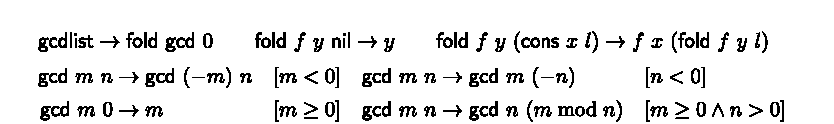
\includegraphics[width=0.95\linewidth,height=0.45\textheight,keepaspectratio]{graphic-01.pdf}\end{center}
 
% END Thmtheorem2.p2
 
% BEGIN Thmtheorem2.p3
 
We use infix notation for some binary operators, and omit logical constraints that are $\mathfrak{t}$. Here is a rewrite sequence: ${\mathsf{gcdlist}}\ {({{\mathsf{cons}}\ {(1+1)}}\ {\mathsf{nil}})}\rightarrow_{\mathcal{R}}{{{\mathsf{fold}}\ {\mathsf{gcd}}}\ {0}}\ {({{\mathsf{cons}}\ {(1+1)}}\ {\mathsf{nil}})}\rightarrow_{\mathcal{R}}{{\mathsf{gcd}}\ {(1+1)}}\ {({{{\mathsf{fold}}\ {\mathsf{gcd}}}\ {0}}\ {\mathsf{nil}})}\rightarrow_{\mathcal{R}}{{\mathsf{gcd}}\ {(1+1)}}\ {0}\rightarrow_{\kappa}{{\mathsf{gcd}}\ {2}}\ {0}\rightarrow_{\mathcal{R}}2$.\par
 
% END Thmtheorem2.p3
 
% END Thmtheorem2
 
% END S2.SS1.SSS0.P0.SPx2
 
% BEGIN S2.SS1.SSS0.P0.SPx3
 
\par\medskip\noindent\textbf{Innermost Rewriting.}\par
 
% BEGIN S2.SS1.SSS0.P0.SPx3.p1
 
The innermost rewrite relation $\xrightarrow{\scriptscriptstyle\mathrm{i}}_{\mathcal{R}}$ requires all the proper subterms of a redex to be in normal form: $t\xrightarrow{\scriptscriptstyle\mathrm{i}}_{\mathcal{R}}t^{\prime}$ if and only if either (1) there exist a context ${C}[]$, a substitution $\sigma$ and a rewrite rule ${\ell}\rightarrow{r}\ [\varphi]\in\mathcal{R}$ such that $t={C}[\ell\sigma]$, $s\not\rightarrow_{\mathcal{R}}s^{\prime}$ for any proper subterm $s$ of $\ell\sigma$ and any $s^{\prime}$, $t^{\prime}={C}[r\sigma]$ and $\sigma$ respects $\varphi$, or (2) $t\rightarrow_{\kappa}t^{\prime}$.\par
 
% END S2.SS1.SSS0.P0.SPx3.p1
 
% BEGIN S2.SS1.SSS0.P0.SPx3.p2
 
Similarly, for an LCSTRS $\mathcal{Q}$ we define the relation $\xrightarrow{\scriptscriptstyle\mathcal{Q}}_{\mathcal{R}}$ as reduction using $\rightarrow_{\mathcal{R}}$ where all proper subterms of a redex are in $\rightarrow_{\mathcal{Q}}$-normal form: $t\xrightarrow{\scriptscriptstyle\mathcal{Q}}_{\mathcal{R}}t^{\prime}$ if and only if either (1) there exist ${C}[]$, $\sigma$ and ${\ell}\rightarrow{r}\ [\varphi]\in\mathcal{R}$ such that $t={C}[\ell\sigma]$, $s\not\rightarrow_{\mathcal{Q}}s^{\prime}$ for any proper subterm $s$ of $\ell\sigma$ and any $s^{\prime}$, $t^{\prime}={C}[r\sigma]$ and $\sigma$ respects $\varphi$, or (2) $t\rightarrow_{\kappa}t^{\prime}$. Note that $\xrightarrow{\scriptscriptstyle\mathrm{i}}_{\mathcal{R}}$ is the same as $\xrightarrow{\scriptscriptstyle\mathcal{R}}_{\mathcal{R}}$.\par
 
% END S2.SS1.SSS0.P0.SPx3.p2
 
% END S2.SS1.SSS0.P0.SPx3
 
% BEGIN S2.SS1.SSS0.P0.SPx4
 
\par\medskip\noindent\textbf{Call-By-Value Rewriting.}\par
 
% BEGIN S2.SS1.SSS0.P0.SPx4.p1
 
We may further restrict a redex by requiring each proper subterm to be a ground term value. Here a term value is either a variable or a term ${\mathsf{f}}\ {{v}_{1}\cdots{v}_{n}}$ where $\mathsf{f}$ is a function symbol, $v_{i}$ is a term value for all $i$, and (1) if there is a rule ${{\mathsf{f}}\ {{t}_{1}\cdots{t}_{k}}}\rightarrow{r}\ [\varphi]\in\mathcal{R}$, then $k>n$; (2) if $\mathsf{f}$ is a calculation symbol, then it takes at least $n+1$ arguments (i.e., $\mathsf{f}:{A}_{1}\rightarrow\cdots\rightarrow{A}_{n+1}\rightarrow B$). In this paper, we will typically refer to term values as just values. By definition, all theory values are values, and all values are in normal form.\par
 
% END S2.SS1.SSS0.P0.SPx4.p1
 
% BEGIN S2.SS1.SSS0.P0.SPx4.p2
 
The definition of the call-by-value rewrite relation $\xrightarrow{\scriptscriptstyle\mathrm{v}}_{\mathcal{R}}$ follows the pattern of $\xrightarrow{\scriptscriptstyle\mathrm{i}}_{\mathcal{R}}$: $t\xrightarrow{\scriptscriptstyle\mathrm{v}}_{\mathcal{R}}t^{\prime}$ if and only if either (1) there exist a context ${C}[]$, a substitution $\sigma$ and a rewrite rule ${\ell}\rightarrow{r}\ [\varphi]\in\mathcal{R}$ such that $t={C}[\ell\sigma]$, $s$ is a ground value for each proper subterm $s$ of $\ell\sigma$, $t^{\prime}={C}[r\sigma]$ and $\sigma$ respects $\varphi$, or (2) $t\rightarrow_{\kappa}t^{\prime}$.\par
 
% END S2.SS1.SSS0.P0.SPx4.p2
 
% BEGIN Thmtheorem3
 
\par\medskip\noindent\textbf{Example 3.}\par
 
% BEGIN Thmtheorem3.p1
 
The rewrite sequence in Example 2 is not innermost (and therefore not call-by-value). An example of a call-by-value rewrite sequence is:\par
 
% END Thmtheorem3.p1
 
% BEGIN Thmtheorem3.p2
 
\begin{center}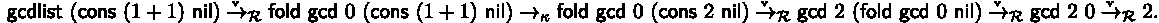
\includegraphics[width=0.95\linewidth,height=0.45\textheight,keepaspectratio]{graphic-02.pdf}\end{center}
 
% END Thmtheorem3.p2
 
% BEGIN Thmtheorem3.p3
 
Note that the redex in the first step is $\mathsf{gcdlist}$, which does not have $1+1$ as subterm.\par
 
% END Thmtheorem3.p3
 
% END Thmtheorem3
 
% BEGIN Thmtheorem4
 
\par\medskip\noindent\textbf{Example 4.}\par
 
% BEGIN Thmtheorem4.p1
 
Consider the LCSTRS $\mathcal{R}=\{{\mathsf{hd}}\ {({{\mathsf{cons}}\ {x}}\ {l})}\rightarrow x,\;{\mathsf{tl}}\ {({{\mathsf{cons}}\ {x}}\ {l})}\rightarrow l\}$. Then the rewrite step ${\mathsf{hd}}\ {({{\mathsf{cons}}\ {42}}\ {({\mathsf{tl}}\ {\mathsf{nil}})})}\xrightarrow{\scriptscriptstyle\mathrm{i}}_{\mathcal{R}}42$ is an innermost step, but not a call-by-value step. The reason is that the subterm ${\mathsf{tl}}\ {\mathsf{nil}}$ of the redex is in normal form, but not a value: innermost rewriting also allows for rewriting above function calls that are not defined on the given arguments; in a language like OCaml, the computation would abort with an error.\par
 
% END Thmtheorem4.p1
 
% END Thmtheorem4
 
% END S2.SS1.SSS0.P0.SPx4
 
% END S2.SS1
 
% BEGIN S2.SS2
 
\par\medskip\noindent\textbf{2.2 Accessibility and Computability}\par
 
% BEGIN S2.SS2.SSS0.P0.SPx1
 
\par\medskip\noindent\textbf{Accessibility.}\par
 
% BEGIN S2.SS2.SSS0.P0.SPx1.p1
 
Assume given a sort ordering – a quasi-ordering $\succsim$ over $\mathcal{S}$ whose strict part ${\succ}={\succsim}\setminus{\precsim}$ is well-founded. We inductively define two relations $\succsim_{+}$ and $\succ_{-}$ over $\mathcal{S}$ and $\mathcal{T}$: for a sort $A$ and a type $B={B}_{1}\rightarrow\cdots\rightarrow{B}_{n}\rightarrow C$ where $C$ is a sort and $n\geq 0$, $A\succsim_{+}B$ if $A\succsim C$ and $A\succ_{-}B_{i}$ for all $i$, and $A\succ_{-}B$ if $A\succ C$ and $A\succsim_{+}B_{i}$ for all $i$.\par
 
% END S2.SS2.SSS0.P0.SPx1.p1
 
% BEGIN S2.SS2.SSS0.P0.SPx1.p2
 
Given a function symbol $\mathsf{f}:{A}_{1}\rightarrow\cdots\rightarrow{A}_{n}\rightarrow B$ where $B$ is a sort, the set $\operatorname{Acc}(\mathsf{f})$ of the accessible argument positions of $\mathsf{f}$ is defined as $\{\,i\,|\,B\succsim_{+}A_{i}\,\}$. A term $t$ is called an accessible subterm of a term $s$, written as $s\trianglerighteq_{\mathrm{acc}}t$, if either $s=t$, or $s={\mathsf{f}}\ {{s}_{1}\cdots{s}_{n}}$ for some $\mathsf{f}\in\mathcal{F}$ and there exists $k\in\operatorname{Acc}(\mathsf{f})$ such that $s_{k}\trianglerighteq_{\mathrm{acc}}t$. An LCSTRS $\mathcal{R}$ is called accessible function passing (AFP) if there exists a sort ordering such that for all ${{\mathsf{f}}\ {{s}_{1}\cdots{s}_{n}}}\rightarrow{r}\ [\varphi]\in\mathcal{R}$ where $\mathsf{f}\in\mathcal{F}$ and $x\in\operatorname{Var}(r)\setminus\operatorname{Var}(\varphi)$, there exists $k$ such that $s_{k}\trianglerighteq_{\mathrm{acc}}x$.\par
 
% END S2.SS2.SSS0.P0.SPx1.p2
 
% BEGIN Thmtheorem5
 
\par\medskip\noindent\textbf{Example 5.}\par
 
% BEGIN Thmtheorem5.p1
 
An LCSTRS $\mathcal{R}$ is AFP (with $\succsim$ equating all the sorts) if for all ${{\mathsf{f}}\ {{s}_{1}\cdots{s}_{n}}}\rightarrow{r}\ [\varphi]\in\mathcal{R}$ where $\mathsf{f}\in\mathcal{F}$ and $i\in\{\,1,\ldots,n\,\}$, the type of each proper subterm of $s_{i}$ is a sort. This is typical for many common examples of higher-order programs manipulating first-order data; e.g., integer recursion or list folding, mapping or filtering; hence, Example 2 is AFP.\par
 
% END Thmtheorem5.p1
 
% BEGIN Thmtheorem5.p2
 
Consider $\{\,{{\mathsf{complst}}\ {\mathsf{fnil}}}\ {x}\rightarrow x,{{\mathsf{complst}}\ {({{\mathsf{fcons}}\ {f}}\ {l})}}\ {x}\rightarrow{{\mathsf{complst}}\ {l}}\ {({f}\ {x})}\,\}$, where $\mathsf{complst}:\mathsf{funlist}\rightarrow\mathsf{int}\rightarrow\mathsf{int}$ composes a list of functions. This system is AFP with $\mathsf{funlist}\succ\mathsf{int}$.\par
 
% END Thmtheorem5.p2
 
% BEGIN Thmtheorem5.p3
 
Consider $\{\,{\mathsf{app}}\ {({\mathsf{lam}}\ {f})}\rightarrow f\,\}$ where $\mathsf{app}:\mathsf{o}\rightarrow\mathsf{o}\rightarrow\mathsf{o}$ and $\mathsf{lam}:(\mathsf{o}\rightarrow\mathsf{o})\rightarrow\mathsf{o}$. This system encodes the untyped lambda-calculus, with $\mathsf{app}$ serving as the application symbol and $\mathsf{lam}$ as a wrapper for abstractions. It is not AFP since $\mathsf{o}\succ\mathsf{o}$ cannot be true.\par
 
% END Thmtheorem5.p3
 
% END Thmtheorem5
 
% END S2.SS2.SSS0.P0.SPx1
 
% BEGIN S2.SS2.SSS0.P0.SPx2
 
\par\medskip\noindent\textbf{Computability.}\par
 
% BEGIN S2.SS2.SSS0.P0.SPx2.p1
 
A term is called neutral if it takes the form ${x}\ {{t}_{1}\cdots{t}_{n}}$ for some variable $x$. A set of reducibility candidates, or an RC-set, for a type-preserving relation $\rightarrow$ over terms – which may stand for $\rightarrow_{\mathcal{R}}$, $\xrightarrow{\scriptscriptstyle\mathrm{i}}_{\mathcal{R}}$, but also $\xrightarrow{\scriptscriptstyle\mathrm{v}}_{\mathcal{R}}$ – is an $\mathcal{S}$-indexed family of sets $(I_{A})_{A\in\mathcal{S}}$ (let $I$ denote $\bigcup_{A}I_{A}$) satisfying the following conditions:\par
  
\par\noindent  (1) 
% BEGIN S2.I2.i1.p1
 
Each element of $I_{A}$ is a terminating (with respect to $\rightarrow$) term of type $A$.\par
 
% END S2.I2.i1.p1
 
 
\par\noindent  (2) 
% BEGIN S2.I2.i2.p1
 
Given terms $s$ and $t$ such that $s\rightarrow t$, if $s$ is in $I_{A}$, so is $t$.\par
 
% END S2.I2.i2.p1
 
 
\par\noindent  (3) 
% BEGIN S2.I2.i3.p1
 
Given a neutral term $s$, if $t$ is in $I_{A}$ for all $t$ such that $s\rightarrow t$, so is $s$.\par
 
% END S2.I2.i3.p1
 
  
A term $t_{0}$ is called $I$-computable if either the type of $t_{0}$ is a sort and $t_{0}\in I$, or the type of $t_{0}$ is $A\rightarrow B$ and ${t_{0}}\ {t_{1}}$ is $I$-computable for all $I$-computable $t_{1}:A$.\par
 
% END S2.SS2.SSS0.P0.SPx2.p1
 
% BEGIN S2.SS2.SSS0.P0.SPx2.p2
 
We are interested in a specific RC-set $\mathbb{C}$:\par
 
% END S2.SS2.SSS0.P0.SPx2.p2
 
% BEGIN Thmtheorem6
 
\par\medskip\noindent\textbf{Theorem 6 (see [13]).}\par
 
% BEGIN Thmtheorem6.p1
 
Given a sort ordering and an RC-set $I$ for $\rightarrow$, let $\Rrightarrow_{I}$ be the relation over terms such that $s\Rrightarrow_{I}t$ if and only if both $s$ and $t$ have a base type, $s={\mathsf{f}}\ {{s}_{1}\cdots{s}_{m}}$ for some function symbol $\mathsf{f}$, $t={s_{k}}\ {{t}_{1}\cdots{t}_{n}}$ for some $k\in\operatorname{Acc}(\mathsf{f})$ and $t_{i}$ is $I$-computable for all $i$.\par
 
% END Thmtheorem6.p1
 
% BEGIN Thmtheorem6.p2
 
Given an LCSTRS $\mathcal{R}$ with a sort ordering, there exists an RC-set $\mathbb{C}$ for $\rightarrow$ such that $t\in\mathbb{C}_{A}$ if and only if $t:A$ is terminating with respect to ${\rightarrow}\cup{\Rrightarrow_{\mathbb{C}}}$, and for all $t^{\prime}$ such that $t\rightarrow^{*}t^{\prime}$, if $t^{\prime}={\mathsf{f}}\ {{t}_{1}\cdots{t}_{n}}$ for some function symbol $\mathsf{f}$, $t_{i}$ is $\mathbb{C}$-computable for all $i\in\operatorname{Acc}(\mathsf{f})$.\par
 
% END Thmtheorem6.p2
 
% END Thmtheorem6
 
% BEGIN S2.SS2.SSS0.P0.SPx2.p3
 
$\mathbb{C}$-computability with respect to the innermost reduction relation $\xrightarrow{\scriptscriptstyle\mathrm{i}}_{\mathcal{R}}$ is at the heart of the soundness proofs for the DP framework defined in this paper (Theorems 14 and 36).\par
 
% END S2.SS2.SSS0.P0.SPx2.p3
 
% END S2.SS2.SSS0.P0.SPx2
 
% END S2.SS2
 
% END S2


% BEGIN S3
 
\par\medskip\noindent\textbf{3 The Transformation of Call-By-Value Systems}\par
 
% BEGIN S3.p1
 
Let us reflect on the shape of call-by-value LCSTRSs. First, we observe that if a pattern $t$ is not a value, neither are its instances, i.e., $t\sigma$ is not a value for any substitution $\sigma$. Hence, under call by value, a rewrite rule ${\ell}\rightarrow{r}\ [\varphi]$ where not all the proper subterms of $\ell$ are values is never applicable, and we can exclude such rewrite rules without loss of generality.\par
 
% END S3.p1
 
% BEGIN S3.p2
 
Second, programming languages hardly allow the addition of constructors to pre-defined (in particular, primitive) data types, such as integers. Given an LCSTRS, in practice, we would also expect, for example, that integer literals are the only constructors for $\mathsf{int}$. Formally, we call a theory sort $B$ inextensible if every function symbol $\mathsf{f}:{A}_{1}\rightarrow\cdots\rightarrow{A}_{n}\rightarrow B$ is a theory symbol or a defined symbol. We do not require that all theory sorts are inextensible; rather, we assume that for each rewrite rule ${\ell}\rightarrow{r}\ [\varphi]$, all the variables in $\operatorname{Var}(\ell)$ whose type is an inextensible theory sort are also in $\operatorname{Var}(\varphi)$. We can do so without loss of generality because such a variable can only be instantiated to a theory value under call by value. We only consider inextensible theory sorts in examples below.\par
 
% END S3.p2
 
% BEGIN S3.p3
 
We write $\varphi,{x}_{1},\ldots,{x}_{n}$ for $\varphi\wedge x_{1}\equiv x_{1}\wedge\cdots\wedge x_{n}\equiv x_{n}$, and conclude the above discussion:\par
 
% END S3.p3
 
% BEGIN Thmtheorem7
 
\par\medskip\noindent\textbf{Lemma 7.}\par
 
% BEGIN Thmtheorem7.p1
 
We apply the below transformation to an LCSTRS $\mathcal{R}$ and let $\mathcal{R}^{\prime}$ be the outcome.\par
  
\par\noindent  (1) 
% BEGIN S3.I1.i1.p1
 
Remove all ${\ell}\rightarrow{r}\ [\varphi]$ where $\ell$ has a proper subterm that is not a value.\par
 
% END S3.I1.i1.p1
 
 
\par\noindent  (2) 
% BEGIN S3.I1.i2.p1
 
Replace all remaining ${\ell}\rightarrow{r}\ [\varphi]$ with ${\ell}\rightarrow{r}\ [\varphi,{x}_{1},\ldots,{x}_{n}]$ where ${x}_{1},\ldots,{x}_{n}$ are the variables in $\operatorname{Var}(\ell)\setminus\operatorname{Var}(\varphi)$ whose type is an inextensible theory sort.\par
 
% END S3.I1.i2.p1
 
  
Then $t\xrightarrow{\scriptscriptstyle\mathrm{v}}_{\mathcal{R}}t^{\prime}$ if and only if $t\xrightarrow{\scriptscriptstyle\mathrm{v}}_{\mathcal{R}^{\prime}}t^{\prime}$ for all $t$ and $t^{\prime}$.\par
 
% END Thmtheorem7.p1
 
% END Thmtheorem7
 
% BEGIN Thmtheorem8
 
\par\medskip\noindent\textbf{Example 8.}\par
 
% BEGIN Thmtheorem8.p1
 
The LCSTRS $\mathcal{R}$ from Example 2 is transformed as follows: (1) no rewrite rules are removed, and (2) four rewrite rules are replaced by the ones below.\par
    $\displaystyle{{{\mathsf{fold}}\ {f}}\ {y}}\ {\mathsf{nil}}$ $\displaystyle\rightarrow y$ $\displaystyle[\mathfrak{t},y]$ $\displaystyle{{\mathsf{gcd}}\ {m}}\ {n}$ $\displaystyle\rightarrow{{\mathsf{gcd}}\ {(-m)}}\ {n}$ $\displaystyle[m<0,n]$     $\displaystyle{{{\mathsf{fold}}\ {f}}\ {y}}\ {({{\mathsf{cons}}\ {x}}\ {l})}$ $\displaystyle\rightarrow{{f}\ {x}}\ {({{{\mathsf{fold}}\ {f}}\ {y}}\ {l})}$ $\displaystyle[\mathfrak{t},x,y]$ $\displaystyle{{\mathsf{gcd}}\ {m}}\ {n}$ $\displaystyle\rightarrow{{\mathsf{gcd}}\ {m}}\ {(-n)}$ $\displaystyle[n<0,m]$    
We will refer to the result of the transformation as $\mathcal{R}_{\mathsf{gcd}}$.\par
 
% END Thmtheorem8.p1
 
% END Thmtheorem8
 
% BEGIN S3.p4
 
We are particularly interested in call-by-value termination. However, innermost termination is more commonly considered in the term rewriting community, and has been studied extensively for first-order term rewriting. In practice, its difference from call-by-value termination is often irrelevant, and their respective techniques are generally similar. Since all values are in normal form, $\xrightarrow{\scriptscriptstyle\mathrm{v}}_{\mathcal{R}}$ is terminating if $\xrightarrow{\scriptscriptstyle\mathrm{i}}_{\mathcal{R}^{\prime}}$ is. Hence, we shall formulate our results in terms of innermost rewriting, for the sake of more generality and less bookkeeping.\par
 
% END S3.p4
 
% END S3


% BEGIN S4
 
\par\medskip\noindent\textbf{4 Static Dependency Pairs and Chains}\par
 
% BEGIN S4.p1
 
The dependency pair method [3] analyzes the recursive structure of function calls. Its variants are at the heart of most modern automatic termination analyzers for various styles of term rewriting. Static dependency pairs [35, 13], a higher-order generalization of the method, are adapted to LCSTRSs in [21]. Now we extend this adaptation for the evaluation strategies.\par
 
% END S4.p1
 
% BEGIN S4.p2
 
First, we recall a notation:\par
 
% END S4.p2
 
% BEGIN Thmtheorem9
 
\par\medskip\noindent\textbf{Definition 9.}\par
 
% BEGIN Thmtheorem9.p1
 
Given an LCSTRS $\mathcal{R}$, let $\mathcal{F}^{\sharp}$ be $\mathcal{F}\uplus\{\,\mathsf{f}^{\sharp}\,|\,\mathsf{f}\in\mathcal{D}\,\}$ where $\mathcal{D}$ is the set of defined symbols in $\mathcal{R}$ and $\mathsf{f}^{\sharp}$ is a fresh function symbol for all $\mathsf{f}$. Let $\mathsf{dp}$ be a fresh sort, and for each defined symbol $\mathsf{f}:{A}_{1}\rightarrow\cdots\rightarrow{A}_{n}\rightarrow B$ where $B\in\mathcal{S}$, we assign $\mathsf{f}^{\sharp}:{A}_{1}\rightarrow\cdots\rightarrow{A}_{n}\rightarrow\mathsf{dp}$. Given a term $t={\mathsf{f}}\ {{t}_{1}\cdots{t}_{n}}\in T(\mathcal{F},\mathcal{V})$ where $\mathsf{f}\in\mathcal{D}$, let $t^{\sharp}$ denote ${\mathsf{f}^{\sharp}}\ {{t}_{1}\cdots{t}_{n}}\in T(\mathcal{F}^{\sharp},\mathcal{V})$.\par
 
% END Thmtheorem9.p1
 
% END Thmtheorem9
 
% BEGIN S4.p3
 
The definition of a static dependency pair is adapted as follows:\par
 
% END S4.p3
 
% BEGIN Thmtheorem10
 
\par\medskip\noindent\textbf{Definition 10.}\par
 
% BEGIN Thmtheorem10.p1
 
A static dependency pair (SDP) is a triple ${s^{\sharp}}\Rightarrow{t^{\sharp}}\ [\varphi]$ where $s^{\sharp}$ and $t^{\sharp}$ are terms of type $\mathsf{dp}$, and $\varphi$ is a logical constraint. This SDP is considered call-by-value if all the proper subterms of $s^{\sharp}$ are values. For a rewrite rule ${\ell}\rightarrow{r}\ [\varphi]$, let $\operatorname{SDP}({\ell}\rightarrow{r}\ [\varphi])$ denote the set of SDPs of form ${{\ell^{\sharp}}\ {{x}_{1}\cdots{x}_{m}}}\Rightarrow{{{\mathsf{g}^{\sharp}}\ {{t}_{1}\cdots{t}_{q}}}\ {{y}_{q+1}\cdots{y}_{n}}}\ [\varphi]$ such that\par
  
\par\noindent  (1) 
% BEGIN S4.I1.i1.p1
 
$\ell^{\sharp}:{A}_{1}\rightarrow\cdots\rightarrow{A}_{m}\rightarrow\mathsf{dp}$ with fresh variables ${x}_{1},\ldots,{x}_{m}$,\par
 
% END S4.I1.i1.p1
 
 
\par\noindent  (2) 
% BEGIN S4.I1.i2.p1
 
${r}\ {{x}_{1}\cdots{x}_{m}}\trianglerighteq{\mathsf{g}}\ {{t}_{1}\cdots{t}_{q}}$ for $\mathsf{g}\in\mathcal{D}$, and\par
 
% END S4.I1.i2.p1
 
 
\par\noindent  (3) 
% BEGIN S4.I1.i3.p1
 
$\mathsf{g}^{\sharp}:{B}_{1}\rightarrow\cdots\rightarrow{B}_{n}\rightarrow\mathsf{dp}$ with fresh variables ${y}_{q+1},\ldots,{y}_{n}$.\par
 
% END S4.I1.i3.p1
 
  
Let $\operatorname{SDP}(\mathcal{R})$ be $\bigcup_{{\ell}\rightarrow{r}\ [\varphi]\in\mathcal{R}}\operatorname{SDP}({\ell}\rightarrow{r}\ [\varphi])$. For ${s^{\sharp}}\Rightarrow{t^{\sharp}}\ [\mathfrak{t}]$, we just write ${s^{\sharp}}\Rightarrow{t^{\sharp}}$.\par
 
% END Thmtheorem10.p1
 
% END Thmtheorem10
 
% BEGIN S4.p4
 
Compared to the quadruple definition in [21], this definition omits the $L$ component, because here its bookkeeping role can be assumed by the logical constraint.\par
 
% END S4.p4
 
% BEGIN S4.p5
 
Intuitively, every dependency pair in $\operatorname{SDP}(\mathcal{R})$ represents a function call in $\mathcal{R}$. If $\mathcal{R}$ is non-terminating, there must be an infinite “chain” of function calls whose arguments are terminating (in other words, the chain is “minimal”: all the proper subterms are terminating). To distinguish the head symbols of those minimal potentially non-terminating terms, we write $\mathsf{f}^{\sharp}$ instead of $\mathsf{f}$ at head positions in SDPs. Then calls to a defined symbol $\mathsf{f}$ (the original) can be assumed to terminate, which is shown separately via $\mathsf{f}^{\sharp}$. And the non-existence of an infinite chain starting from a call to any $\mathsf{f}^{\sharp}$ in $\operatorname{SDP}(\mathcal{R})$ implies the termination of $\mathcal{R}$.\par
 
% END S4.p5
 
% BEGIN Thmtheorem11
 
\par\medskip\noindent\textbf{Example 11.}\par
 
% BEGIN Thmtheorem11.p1
 
Following Example 8, $\operatorname{SDP}(\mathcal{R}_{\mathsf{gcd}})$ consists of the following SDPs:\par
  
\par\noindent  (1) 
% BEGIN S4.I2.i1.p1
 
${{\mathsf{gcdlist}^{\sharp}}\ {l^{\prime}}}\Rightarrow{{{\mathsf{gcd}^{\sharp}}\ {m^{\prime}}}\ {n^{\prime}}}$\par
 
% END S4.I2.i1.p1
 
 
\par\noindent  (2) 
% BEGIN S4.I2.i2.p1
 
${{\mathsf{gcdlist}^{\sharp}}\ {l^{\prime}}}\Rightarrow{{{{\mathsf{fold}^{\sharp}}\ {\mathsf{gcd}}}\ {0}}\ {l^{\prime}}}$\par
 
% END S4.I2.i2.p1
 
 
\par\noindent  (3) 
% BEGIN S4.I2.i3.p1
 
${{{\mathsf{gcd}^{\sharp}}\ {m}}\ {n}}\Rightarrow{{{\mathsf{gcd}^{\sharp}}\ {(-m)}}\ {n}}\ [m<0,n]$\par
 
% END S4.I2.i3.p1
 
 
\par\noindent  (4) 
% BEGIN S4.I2.i4.p1
 
${{{\mathsf{gcd}^{\sharp}}\ {m}}\ {n}}\Rightarrow{{{\mathsf{gcd}^{\sharp}}\ {m}}\ {(-n)}}\ [n<0,m]$\par
 
% END S4.I2.i4.p1
 
 
\par\noindent  (5) 
% BEGIN S4.I2.i5.p1
 
${{{\mathsf{gcd}^{\sharp}}\ {m}}\ {n}}\Rightarrow{{{\mathsf{gcd}^{\sharp}}\ {n}}\ {(m\bmod n)}}\ [m\geq 0\wedge n>0]$\par
 
% END S4.I2.i5.p1
 
 
\par\noindent  (6) 
% BEGIN S4.I2.i6.p1
 
${{{{\mathsf{fold}^{\sharp}}\ {f}}\ {y}}\ {({{\mathsf{cons}}\ {x}}\ {l})}}\Rightarrow{{{{\mathsf{fold}^{\sharp}}\ {f}}\ {y}}\ {l}}\ [\mathfrak{t},x,y]$\par
 
% END S4.I2.i6.p1
 
  
% END Thmtheorem11.p1
 
% END Thmtheorem11
 
% BEGIN S4.p6
 
In this paper, a set $\mathcal{R}$ of rewrite rules plays two roles: (1) it specifies how to rewrite arguments in SDPs, and (2) it determines which rewrite steps are innermost and which terms are values. In Sections 5 and 6, a given set $\mathcal{R}$ in its first role may be modified (with rewrite rules removed). In this process, if we do not keep the original set, there can be unintended consequences for its second role. For example, consider $\mathcal{R}=\{\,{\mathsf{f}}\ {x}\rightarrow r_{1},\mathsf{a}\rightarrow r_{2}\,\}$. Note that the first rewrite rule is not applicable to ${\mathsf{f}}\ {\mathsf{a}}$ with respect to innermost rewriting. Now if we remove the second rewrite rule from $\mathcal{R}$ and consider the new set, the remaining rewrite rule will be applicable, and the term $\mathsf{a}$ will be a value, which is generally an unwanted change.\par
 
% END S4.p6
 
% BEGIN S4.p7
 
Hence, we keep a copy of the original set $\mathcal{R}$ of rewrite rules to faithfully determine which rewrite steps are innermost and which terms are values. Following [18, 41], we let $\mathcal{Q}$ denote this copy. In contrast to the literature, we consider $\mathcal{Q}$ fixed throughout the analysis of a given system.444A fixed set $\mathcal{Q}$ suffices in this paper because our DP processors may remove rewrite rules, but may not add new rewrite rules or change the signature (e.g., with semantic labeling [45]). Now we formalize the idea of a chain of function calls in the innermost setting:\par
 
% END S4.p7
 
% BEGIN Thmtheorem12
 
\par\medskip\noindent\textbf{Definition 12.}\par
 
% BEGIN Thmtheorem12.p1
 
Given a set $\mathcal{P}$ of SDPs and a set $\mathcal{R}$ of rewrite rules, an innermost $(\mathcal{P},\mathcal{R})$-chain is a (finite or infinite) sequence $({s_{0}^{\sharp}}\Rightarrow{t_{0}^{\sharp}}\ [\varphi_{0}],\sigma_{0}),({s_{1}^{\sharp}}\Rightarrow{t_{1}^{\sharp}}\ [\varphi_{1}],\sigma_{1}),\ldots$ such that for all $i$, ${s_{i}^{\sharp}}\Rightarrow{t_{i}^{\sharp}}\ [\varphi_{i}]\in\mathcal{P}$, $\sigma_{i}$ is a substitution which respects $\varphi_{i}$, $s_{i}^{\sharp}\sigma_{i}$ is in normal form with respect to $\rightarrow_{\mathcal{Q}}$, and $t_{i-1}^{\sharp}\sigma_{i-1}\xrightarrow{\scriptscriptstyle\mathcal{Q}}_{\mathcal{R}}^{*}s_{i}^{\sharp}\sigma_{i}$ if $i>0$.\par
 
% END Thmtheorem12.p1
 
% END Thmtheorem12
 
% BEGIN Thmtheorem13
 
\par\medskip\noindent\textbf{Example 13.}\par
 
% BEGIN Thmtheorem13.p1
 
Following Example 11, $(\text{1},[{l^{\prime}}\coloneq{\mathsf{nil}},{m^{\prime}}\coloneq{24},{n^{\prime}}\coloneq{18}]),(\text{5},[{m}\coloneq{24},{n}\coloneq{18}]),(\text{5},[{m}\coloneq{18},{n}\coloneq{6}])$ is an innermost $(\operatorname{SDP}(\mathcal{R}_{\mathsf{gcd}}),\mathcal{R}_{\mathsf{gcd}})$-chain.\par
 
% END Thmtheorem13.p1
 
% END Thmtheorem13
 
% BEGIN S4.p8
 
In the above definition, the requirement that $s_{i}^{\sharp}\sigma_{i}$ is in normal form implies that $\sigma_{i}(x)$ is in normal form for all $x\in\operatorname{Var}(s_{i}^{\sharp})$, including fresh variables such as $l^{\prime}$ in SDP (1). Hence, the call-by-value (and therefore innermost) rewrite sequence in Example 3 does not directly translate to an innermost $(\operatorname{SDP}(\mathcal{R}),\mathcal{R})$-chain. Nevertheless, we have the following result:\par
 
% END S4.p8
 
% BEGIN Thmtheorem14
 
\par\medskip\noindent\textbf{Theorem 14.}\par
 
% BEGIN Thmtheorem14.p1
 
An AFP system $\mathcal{R}$ is innermost (and therefore call-by-value) terminating if there exists no infinite innermost $(\operatorname{SDP}(\mathcal{R}),\mathcal{R})$-chain.\par
 
% END Thmtheorem14.p1
 
% END Thmtheorem14
 
% BEGIN S4.SS0.SSS0.P0.SPx1
 
\par\medskip\noindent\textbf{Proof Idea.}\par
 
% BEGIN S4.SS0.SSS0.P0.SPx1.p1
 
The full proof is in Section A.2, and is very similar to its counterpart for termination with respect to full rewriting [21]: in a non-terminating LCSTRS, we can always identify a non-terminating base-type term $t={\mathsf{f}}\ {{t}_{1}\cdots{t}_{n}}$ such that all $t_{i}$ are $\mathbb{C}$-computable; and from an infinite reduction $t\xrightarrow{\scriptscriptstyle\mathrm{i}}_{\mathcal{R}}t^{\prime}\xrightarrow{\scriptscriptstyle\mathrm{i}}_{\mathcal{R}}t^{\prime\prime}\xrightarrow{\scriptscriptstyle\mathrm{i}}_{\mathcal{R}}\dots$ we can find $s,u$ such that $s={\mathsf{f}}\ {(t_{1}\,{\downarrow}_{\mathcal{R}})\cdots(t_{n}\,{\downarrow}_{\mathcal{R}})}$, $(s^{\sharp},u^{\sharp})$ is an instance of a dependency pair, and $u$ is again non-terminating with $\mathbb{C}$-computable arguments. The primary difference from [21] is the need to ensure all variables are instantiated to normal forms, which for the fresh variables discussed above means that we must choose the right normal form that still yields non-termination. $\hfill\blacktriangleleft$\par
 
% END S4.SS0.SSS0.P0.SPx1.p1
 
% END S4.SS0.SSS0.P0.SPx1
 
% END S4


% BEGIN S5
 
\par\medskip\noindent\textbf{5 The Innermost DP Framework}\par
 
% BEGIN S5.p1
 
In this section, we modify the constrained DP framework [21] to prove innermost termination. The DP framework is a collection of DP processors, each of which represents a technique.\par
 
% END S5.p1
 
% BEGIN Thmtheorem15
 
\par\medskip\noindent\textbf{Definition 15.}\par
 
% BEGIN Thmtheorem15.p1
 
A DP problem is a pair $(\mathcal{P},\mathcal{R})$ where $\mathcal{P}$ is a set of SDPs and $\mathcal{R}$ is a set of rewrite rules. If no infinite innermost $(\mathcal{P},\mathcal{R})$-chain exists, $(\mathcal{P},\mathcal{R})$ is called finite. A DP processor is a partial mapping which possibly assigns to a DP problem a set of DP problems. A DP processor $\rho$ is called sound if $(\mathcal{P},\mathcal{R})$ is finite whenever all the elements of $\rho(\mathcal{P},\mathcal{R})$ are.\par
 
% END Thmtheorem15.p1
 
% END Thmtheorem15
 
% BEGIN S5.p2
 
Theorem 14 tells us that an AFP system $\mathcal{R}$ is innermost terminating if $(\operatorname{SDP}(\mathcal{R}),\mathcal{R})$ is a finite DP problem. Given a collection of sound DP processors, we have the following procedure: (1) $\mathcal{Q}\coloneq\mathcal{R}$, $S\coloneq\{\,(\operatorname{SDP}(\mathcal{R}),\mathcal{R})\,\}$; (2) while $S$ contains a DP problem $(\mathcal{P},\mathcal{R})$ to which some sound DP processor $\rho$ is applicable, $S\coloneq(S\setminus\{\,(\mathcal{P},\mathcal{R})\,\})\cup\rho(\mathcal{P},\mathcal{R})$. If this procedure ends with $S=\emptyset$, we can conclude that $\mathcal{R}$ is innermost terminating.\par
 
% END S5.p2
 
% BEGIN S5.SS1
 
\par\medskip\noindent\textbf{5.1 Graph, Subterm Criterion and Integer Mapping Processors}\par
 
% BEGIN S5.SS1.p1
 
Three classes of DP processors in [21] remain essentially unchanged in the innermost setting. Let us review their application to the system $\mathcal{R}_{\mathsf{gcd}}$ from Example 8, which is discussed by [21] in the form of Example 2. First, we consider a graph approximation for $(\operatorname{SDP}(\mathcal{R}_{\mathsf{gcd}}),\mathcal{R}_{\mathsf{gcd}})$:\par
 
% END S5.SS1.p1
 
% BEGIN Thmtheorem16
 
\par\medskip\noindent\textbf{Definition 16.}\par
 
% BEGIN Thmtheorem16.p1
 
For a DP problem $(\mathcal{P},\mathcal{R})$, a graph approximation $(G,\theta)$ consists of a finite directed graph $G$ and a mapping $\theta$ from $\mathcal{P}$ to the vertices of $G$ such that there is an edge from $\theta(p_{0})$ to $\theta(p_{1})$ whenever $(p_{0},\sigma_{0}),(p_{1},\sigma_{1})$ is an innermost $(\mathcal{P},\mathcal{R})$-chain for some $\sigma_{0}$ and $\sigma_{1}$.\par
 
% END Thmtheorem16.p1
 
% END Thmtheorem16
 
% BEGIN S5.SS1.p2
 
Compared to [21], the main change is that we now check for innermost $(\mathcal{P},\mathcal{R})$-chains to determine which edges must exist. A graph approximation for $(\operatorname{SDP}(\mathcal{R}_{\mathsf{gcd}}),\mathcal{R}_{\mathsf{gcd}})$ is in Figure 1. Despite the slightly different SDPs (due to the transformation of the call-by-value system), this graph approximation is the same as the one in [21].\par
 
% END S5.SS1.p2
 
% BEGIN S5.F1

\begin{center}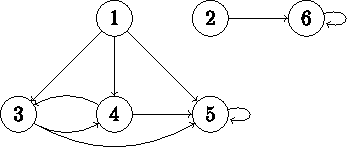
\includegraphics[width=0.95\linewidth,height=0.45\textheight,keepaspectratio]{graphic-03.pdf}\end{center}
 
Figure 1: A graph approximation for $(\operatorname{SDP}(\mathcal{R}_{\mathsf{gcd}}),\mathcal{R}_{\mathsf{gcd}})$.\par
 
% END S5.F1
 
% BEGIN S5.SS1.p3
 
Given a graph approximation, we can decompose the DP problem:\par
 
% END S5.SS1.p3
 
% BEGIN Thmtheorem17
 
\par\medskip\noindent\textbf{Definition 17.}\par
 
% BEGIN Thmtheorem17.p1
 
Given a DP problem $(\mathcal{P},\mathcal{R})$, a graph processor computes a graph approximation $(G,\theta)$ for $(\mathcal{P},\mathcal{R})$ and the strongly connected components (SCCs) of $G$, then returns $\{\,(\{\,p\in\mathcal{P}\,|\,\theta(p)\text{ belongs to }S\,\},\mathcal{R})\,|\,S\text{ is a non-trivial SCC of }G\,\}$.\par
 
% END Thmtheorem17.p1
 
% END Thmtheorem17
 
% BEGIN S5.SS1.p4
 
If a graph processor produces the graph approximation in Figure 1, it will return the set $\{\,(\{\,\text{6}\,\},\mathcal{R}_{\mathsf{gcd}}),(\{\,\text{3},\text{4}\,\},\mathcal{R}_{\mathsf{gcd}}),(\{\,\text{5}\,\},\mathcal{R}_{\mathsf{gcd}})\,\}$. Next, we observe that $\mathsf{fold}$ is defined by structural recursion, which can be handled by subterm criterion processors. Let $\operatorname{heads}(\mathcal{P})$ denote the set of function symbols heading either side of an SDP in $\mathcal{P}$, and we have the following definition:\par
 
% END S5.SS1.p4
 
% BEGIN Thmtheorem18
 
\par\medskip\noindent\textbf{Definition 18.}\par
 
% BEGIN Thmtheorem18.p1
 
A projection $\nu$ for a set $\mathcal{P}$ of SDPs is a mapping from $\operatorname{heads}(\mathcal{P})$ to integers such that $1\leq\nu(\mathsf{f}^{\sharp})\leq n$ if $\mathsf{f}^{\sharp}:{A}_{1}\rightarrow\cdots\rightarrow{A}_{n}\rightarrow\mathsf{dp}$. Let $\bar{\nu}({\mathsf{f}^{\sharp}}\ {{t}_{1}\cdots{t}_{n}})$ denote $t_{\nu(\mathsf{f}^{\sharp})}$. A projection $\nu$ is said to $\vartriangleright$-orient a subset $\mathcal{P}^{\prime}$ of $\mathcal{P}$ if $\bar{\nu}(s^{\sharp})\vartriangleright\bar{\nu}(t^{\sharp})$ for all ${s^{\sharp}}\Rightarrow{t^{\sharp}}\ [\varphi]\in\mathcal{P}^{\prime}$ and $\bar{\nu}(s^{\sharp})=\bar{\nu}(t^{\sharp})$ for all ${s^{\sharp}}\Rightarrow{t^{\sharp}}\ [\varphi]\in\mathcal{P}\setminus\mathcal{P}^{\prime}$. A subterm criterion processor maps $(\mathcal{P},\mathcal{R})$ to $\{\,(\mathcal{P}\setminus\mathcal{P}^{\prime},\mathcal{R})\,\}$ for some non-empty $\mathcal{P}^{\prime}\subseteq\mathcal{P}$ which is $\vartriangleright$-oriented by some projection for $\mathcal{P}$.\par
 
% END Thmtheorem18.p1
 
% END Thmtheorem18
 
% BEGIN S5.SS1.p5
 
Choosing $\nu(\mathsf{fold}^{\sharp})=3$, we have $\bar{\nu}({{{\mathsf{fold}^{\sharp}}\ {f}}\ {y}}\ {({{\mathsf{cons}}\ {x}}\ {l})})={{\mathsf{cons}}\ {x}}\ {l}\vartriangleright l=\bar{\nu}({{{\mathsf{fold}^{\sharp}}\ {f}}\ {y}}\ {l})$, so a subterm criterion processor maps $(\{\,\text{6}\,\},\mathcal{R}_{\mathsf{gcd}})$ to $\{\,(\emptyset,\mathcal{R}_{\mathsf{gcd}})\,\}$, and $(\emptyset,\mathcal{R}_{\mathsf{gcd}})$ can (trivially) be removed by a graph processor. Now we are left with $(\{\,\text{3},\text{4}\,\},\mathcal{R}_{\mathsf{gcd}})$ and $(\{\,\text{5}\,\},\mathcal{R}_{\mathsf{gcd}})$, which involve recursion over integers. We deal with those by means of integer mappings:\par
 
% END S5.SS1.p5
 
% BEGIN Thmtheorem19
 
\par\medskip\noindent\textbf{Definition 19.}\par
 
% BEGIN Thmtheorem19.p1
 
Given a set $\mathcal{P}$ of SDPs, for all $\mathsf{f}^{\sharp}\in\operatorname{heads}(\mathcal{P})$ where $\mathsf{f}^{\sharp}:{A}_{1}\rightarrow\cdots\rightarrow{A}_{n}\rightarrow\mathsf{dp}$, let $\iota(\mathsf{f}^{\sharp})$ be the subset of $\{\,1,\ldots,n\,\}$ such that $i\in\iota(\mathsf{f}^{\sharp})$ if and only if $A_{i}\in{\mathcal{S}}_{\vartheta}$ and the $i$-th argument of any occurrence of $\mathsf{f}^{\sharp}$ in an SDP ${s^{\sharp}}\Rightarrow{t^{\sharp}}\ [\varphi]\in\mathcal{P}$ is in $T({\mathcal{F}}_{\vartheta},\operatorname{Var}(\varphi))$. Let $\mathcal{X}(\mathsf{f}^{\sharp})$ be a set of fresh variables $\{\,x_{i}\,|\,i\in\iota(\mathsf{f}^{\sharp})\,\}$ where $x_{i}:A_{i}$ for all $i$. An integer mapping $\mathcal{J}$ for $\mathcal{P}$ is a mapping from $\operatorname{heads}(\mathcal{P})$ to theory terms such that for all $\mathsf{f}^{\sharp}$, $\mathcal{J}(\mathsf{f}^{\sharp}):\mathsf{int}$ and $\operatorname{Var}(\mathcal{J}(\mathsf{f}^{\sharp}))\subseteq\mathcal{X}(\mathsf{f}^{\sharp})$. Let $\bar{\mathcal{J}}({\mathsf{f}^{\sharp}}\ {{t}_{1}\cdots{t}_{n}})$ denote $\mathcal{J}(\mathsf{f}^{\sharp})[{x_{i}}\coloneq{t_{i}}]_{i\in\iota(\mathsf{f}^{\sharp})}$.\par
 
% END Thmtheorem19.p1
 
% END Thmtheorem19
 
% BEGIN S5.SS1.p6
 
Integer mapping processors handle decreasing integer values:\par
 
% END S5.SS1.p6
 
% BEGIN Thmtheorem20
 
\par\medskip\noindent\textbf{Definition 20.}\par
 
% BEGIN Thmtheorem20.p1
 
Given a set $\mathcal{P}$ of SDPs, an integer mapping $\mathcal{J}$ is said to $>$-orient a subset $\mathcal{P}^{\prime}$ of $\mathcal{P}$ if $\varphi\models\bar{\mathcal{J}}(s^{\sharp})\geq 0\wedge\bar{\mathcal{J}}(s^{\sharp})>\bar{\mathcal{J}}(t^{\sharp})$ for all ${s^{\sharp}}\Rightarrow{t^{\sharp}}\ [\varphi]\in\mathcal{P}^{\prime}$, and $\varphi\models\bar{\mathcal{J}}(s^{\sharp})\geq\bar{\mathcal{J}}(t^{\sharp})$ for all ${s^{\sharp}}\Rightarrow{t^{\sharp}}\ [\varphi]\in\mathcal{P}\setminus\mathcal{P}^{\prime}$, where $\varphi\models\varphi^{\prime}$ denotes that $[\![\varphi\sigma]\!]=1$ implies $[\![\varphi^{\prime}\sigma]\!]=1$ for each substitution $\sigma$ which maps variables in $\operatorname{Var}(\varphi)\cup\operatorname{Var}(\varphi^{\prime})$ to theory values. An integer mapping processor maps $(\mathcal{P},\mathcal{R})$ to $\{\,(\mathcal{P}\setminus\mathcal{P}^{\prime},\mathcal{R})\,\}$ for some non-empty $\mathcal{P}^{\prime}\subseteq\mathcal{P}$ which is $>$-oriented by some integer mapping for $\mathcal{P}$.\par
 
% END Thmtheorem20.p1
 
% END Thmtheorem20
 
% BEGIN S5.SS1.p7
 
To deal with $(\{\,\text{5}\,\},\mathcal{R}_{\mathsf{gcd}})$, let $\mathcal{J}(\mathsf{gcd}^{\sharp})$ be $x_{2}$ so $\bar{\mathcal{J}}({{\mathsf{gcd}^{\sharp}}\ {m}}\ {n})=n$, $\bar{\mathcal{J}}({{\mathsf{gcd}^{\sharp}}\ {n}}\ {(m\bmod n)})=m\bmod n$ and $m\geq 0\wedge n>0\models n\geq 0\wedge n>m\bmod n$. Then an integer mapping processor returns $\{\,(\emptyset,\mathcal{R}_{\mathsf{gcd}})\,\}$, and $(\emptyset,\mathcal{R}_{\mathsf{gcd}})$ can (trivially) be removed by a graph processor.\par
 
% END S5.SS1.p7
 
% BEGIN S5.SS1.p8
 
Unlike [21], here an integer mapping processor is applicable to $(\{\,\text{3},\text{4}\,\},\mathcal{R}_{\mathsf{gcd}})$: $\mathcal{J}(\mathsf{gcd}^{\sharp})={-x_{1}}$ and the processor returns $\{\,(\{\,\text{4}\,\},\mathcal{R}_{\mathsf{gcd}})\,\}$. Then $(\{\,\text{4}\,\},\mathcal{R}_{\mathsf{gcd}})$ can be removed by a graph processor. This simpler proof is due to the transformation of the call-by-value system; in both SDPs, $m$ and $n$ can be instantiated only to theory values, which is not the case in [21], and a theory argument processor is needed there. To elaborate, we consider the system $\mathcal{R}$:\par
    \[{{{\mathsf{f}}\ {x}}\ {y}}\ {z}\rightarrow{{{\mathsf{f}}\ {x}}\ {(x+1)}}\ {(x-1)}\quad[y<z]\qquad{{\mathsf{c}}\ {x}}\ {y}\rightarrow x\qquad{{\mathsf{c}}\ {x}}\ {y}\rightarrow y\]    
We have ${{{\mathsf{f}}\ {({{\mathsf{c}}\ {0}}\ {3})}}\ {1}}\ {2}\rightarrow_{\mathcal{R}}{{{\mathsf{f}}\ {({{\mathsf{c}}\ {0}}\ {3})}}\ {(({{\mathsf{c}}\ {0}}\ {3})+1)}}\ {(({{\mathsf{c}}\ {0}}\ {3})-1)}\rightarrow_{\mathcal{R}}^{+}{{{\mathsf{f}}\ {({{\mathsf{c}}\ {0}}\ {3})}}\ {1}}\ {2}$, and therefore $\mathcal{R}$ is not terminating with respect to full rewriting. Under call by value, $\mathcal{R}$ is terminating: the first rewrite rule with $x$ appended to the logical constraint gives the only SDP ${{{{\mathsf{f}^{\sharp}}\ {x}}\ {y}}\ {z}}\Rightarrow{{{{\mathsf{f}^{\sharp}}\ {x}}\ {(x+1)}}\ {(x-1)}}\ [y<z,x]$, then let $\mathcal{J}(\mathsf{f}^{\sharp})$ be $x_{3}-x_{2}$. Here we benefit from call by value.\par
 
% END S5.SS1.p8
 
% END S5.SS1
 
% BEGIN S5.SS2
 
\par\medskip\noindent\textbf{5.2 The Chaining of Call-By-Value SDPs}\par
 
% BEGIN S5.SS2.p1
 
Another benefit of call by value is that we may chain together consecutive SDPs, e.g., ${{\mathsf{fact}^{\sharp}}\ {x}}\Rightarrow{{{\mathsf{u}_{1}^{\sharp}}\ {x}}\ {1}}\ [\mathfrak{t},x]$ and ${{{\mathsf{u}_{1}^{\sharp}}\ {x}}\ {z}}\Rightarrow{{{{\mathsf{u}_{2}^{\sharp}}\ {x}}\ {z}}\ {1}}\ [\mathfrak{t},x,z]$ may merge to form ${{\mathsf{fact}^{\sharp}}\ {x}}\Rightarrow{{{{\mathsf{u}_{2}^{\sharp}}\ {x}}\ {1}}\ {1}}\ [\mathfrak{t},x]$. This capability can be important for automatically generated systems.\par
 
% END S5.SS2.p1
 
% BEGIN Thmtheorem21
 
\par\medskip\noindent\textbf{Definition 21.}\par
 
% BEGIN Thmtheorem21.p1
 
Given SDPs $p_{0}=({s_{0}^{\sharp}}\Rightarrow{{\mathsf{f}^{\sharp}}\ {{t^{\prime}}_{1}\cdots{t^{\prime}}_{n}}}\ [\varphi_{0}])$ and $p_{1}=({{\mathsf{f}^{\sharp}}\ {{s^{\prime}}_{1}\cdots{s^{\prime}}_{n}}}\Rightarrow{t_{1}^{\sharp}}\ [\varphi_{1}])$ where $\mathsf{f}\in\mathcal{D}$ and variables are renamed if necessary to avoid name collisions, $p_{0}$ and $p_{1}$ are called chainable if $p_{1}$ is a call-by-value SDP and there exists a substitution $\sigma$ such that $\operatorname{dom}(\sigma)=\bigcup_{i=1}^{n}\operatorname{Var}(s_{i}^{\prime})$, $t_{i}^{\prime}=s_{i}^{\prime}\sigma$ for all $i$, and $\sigma(x)\in T({\mathcal{F}}_{\vartheta},\operatorname{Var}(\varphi_{0}))$ for all $x\in\operatorname{dom}(\sigma)\cap\operatorname{Var}(\varphi_{1})$. The chaining $\operatorname{ch}(p_{0},p_{1})$ of $p_{0}$ and $p_{1}$ is ${s_{0}^{\sharp}}\Rightarrow{t_{1}^{\sharp}\sigma}\ [\varphi_{0}\wedge(\varphi_{1}\sigma)]$.\par
 
% END Thmtheorem21.p1
 
% END Thmtheorem21
 
% BEGIN S5.SS2.p2
 
Note that in the context of call-by-value rewriting, all SDPs can be assumed to be call-by-value, and therefore it is not particularly restrictive to so require $p_{1}$ above. To see the importance of this requirement, consider the DP problem $(\{\,{{{\mathsf{f}^{\sharp}}\ {\mathsf{a}}}\ {\mathsf{b}}}\Rightarrow{{\mathsf{g}^{\sharp}}\ {({{\mathsf{h}}\ {\mathsf{b}}}\ {\mathsf{a}})}},{{\mathsf{g}^{\sharp}}\ {({{\mathsf{h}}\ {x}}\ {y})}}\Rightarrow{{{\mathsf{f}^{\sharp}}\ {x}}\ {y}}\,\},\{\,{{\mathsf{h}}\ {\mathsf{b}}}\ {\mathsf{a}}\rightarrow{{\mathsf{h}}\ {\mathsf{a}}}\ {\mathsf{b}}\,\})$. If we dropped the call-by-value requirement for the second SDP, the two SDPs would be chainable and yield ${{{\mathsf{f}^{\sharp}}\ {\mathsf{a}}}\ {\mathsf{b}}}\Rightarrow{{{\mathsf{f}^{\sharp}}\ {\mathsf{b}}}\ {\mathsf{a}}}$. However, ${{\mathsf{f}^{\sharp}}\ {\mathsf{b}}}\ {\mathsf{a}}$ is not reachable from ${{\mathsf{f}^{\sharp}}\ {\mathsf{a}}}\ {\mathsf{b}}$ initially, and replacing the original SDPs with the new one is not sound.\par
 
% END S5.SS2.p2
 
% BEGIN Thmtheorem22
 
\par\medskip\noindent\textbf{Definition 22.}\par
 
% BEGIN Thmtheorem22.p1
 
Given a set $\mathcal{P}$ of SDPs and $\mathsf{f}\in\mathcal{D}$ such that $\mathcal{P}_{\mathsf{f}}^{\ell}\neq\emptyset$, $\mathcal{P}_{\mathsf{f}}^{r}\neq\emptyset$, $\mathcal{P}_{\mathsf{f}}^{\ell}\cap\mathcal{P}_{\mathsf{f}}^{r}=\emptyset$ and every pair in $\mathcal{P}_{\mathsf{f}}^{r}\times\mathcal{P}_{\mathsf{f}}^{\ell}$ is chainable where $\mathcal{P}_{\mathsf{f}}^{\ell}=\{\,{s^{\sharp}}\Rightarrow{t^{\sharp}}\ [\varphi]\in\mathcal{P}\,|\,s^{\sharp}={\mathsf{f}^{\sharp}}\ {{s}_{1}\cdots{s}_{n}}\,\}$ and $\mathcal{P}_{\mathsf{f}}^{r}=\{\,{s^{\sharp}}\Rightarrow{t^{\sharp}}\ [\varphi]\in\mathcal{P}\,|\,t^{\sharp}={\mathsf{f}^{\sharp}}\ {{t}_{1}\cdots{t}_{n}}\,\}$, a chaining processor assigns to a DP problem $(\mathcal{P},\mathcal{R})$ the singleton $\{\,((\mathcal{P}\setminus(\mathcal{P}_{\mathsf{f}}^{\ell}\cup\mathcal{P}_{\mathsf{f}}^{r}))\cup\mathcal{P}^{\prime},\mathcal{R})\,\}$ where $\mathcal{P}^{\prime}=\{\,\operatorname{ch}(p_{0},p_{1})\,|\,p_{0}\in\mathcal{P}_{\mathsf{f}}^{r}\text{ and }p_{1}\in\mathcal{P}_{\mathsf{f}}^{\ell}\,\}$.\par
 
% END Thmtheorem22.p1
 
% END Thmtheorem22
 
% BEGIN Thmtheorem23
 
\par\medskip\noindent\textbf{Example 23.}\par
 
% BEGIN Thmtheorem23.p1
 
Consider the below set $\mathcal{P}$ of SDPs generated from an imperative program [14]:\par
    $\displaystyle{\mathsf{fact}^{\sharp}}\ {x}$ $\displaystyle\Rightarrow{{\mathsf{u}_{1}^{\sharp}}\ {x}}\ {1}$ $\displaystyle[\mathfrak{t},x]$ $\displaystyle{{\mathsf{u}_{1}^{\sharp}}\ {x}}\ {z}$ $\displaystyle\Rightarrow{{{\mathsf{u}_{2}^{\sharp}}\ {x}}\ {z}}\ {1}$ $\displaystyle[\mathfrak{t},x,z]$     $\displaystyle{{{\mathsf{u}_{2}^{\sharp}}\ {x}}\ {z}}\ {i}$ $\displaystyle\Rightarrow{{{\mathsf{u}_{3}^{\sharp}}\ {x}}\ {z}}\ {i}$ $\displaystyle[i\leq x,z]$ $\displaystyle{{{\mathsf{u}_{3}^{\sharp}}\ {x}}\ {z}}\ {i}$ $\displaystyle\Rightarrow{{{\mathsf{u}_{4}^{\sharp}}\ {x}}\ {(z*i)}}\ {i}$ $\displaystyle[\mathfrak{t},x,z,i]$     $\displaystyle{{{\mathsf{u}_{2}^{\sharp}}\ {x}}\ {z}}\ {i}$ $\displaystyle\Rightarrow{{\mathsf{u}_{5}^{\sharp}}\ {x}}\ {z}$ $\displaystyle[\neg(i\leq x),z]$ $\displaystyle{{{\mathsf{u}_{4}^{\sharp}}\ {x}}\ {z}}\ {i}$ $\displaystyle\Rightarrow{{{\mathsf{u}_{2}^{\sharp}}\ {x}}\ {z}}\ {(i+1)}$ $\displaystyle[\mathfrak{t},x,z,i]$    
Chaining processors can iteratively remove the occurrences of $\mathsf{u}_{1}^{\sharp}$, $\mathsf{u}_{3}^{\sharp}$ and $\mathsf{u}_{4}^{\sharp}$, and end with (1) ${{\mathsf{fact}^{\sharp}}\ {x}}\Rightarrow{{{{\mathsf{u}_{2}^{\sharp}}\ {x}}\ {1}}\ {1}}\ [\mathfrak{t},x]$, (2) ${{{{\mathsf{u}_{2}^{\sharp}}\ {x}}\ {z}}\ {i}}\Rightarrow{{{{\mathsf{u}_{2}^{\sharp}}\ {x}}\ {(z*i)}}\ {(i+1)}}\ [i\leq x,z]$, and (3) ${{{{\mathsf{u}_{2}^{\sharp}}\ {x}}\ {z}}\ {i}}\Rightarrow{{{\mathsf{u}_{5}^{\sharp}}\ {x}}\ {z}}\ [\neg(i\leq x),z]$. Note that a chaining processor for $\mathsf{f}\in\mathcal{D}$ removes all the occurrences of $\mathsf{f}^{\sharp}$ in $\mathcal{P}$, and therefore the process of iteratively applying chaining processors always terminates (on the assumption that $\operatorname{heads}(\mathcal{P})$ is finite). In this example, the above outcome cannot be further chained; there is no chaining processor for $\mathsf{u}_{2}$ because $\mathcal{P}_{\mathsf{u}_{2}}^{\ell}\cap\mathcal{P}_{\mathsf{u}_{2}}^{r}$ contains SDP (23).\par
 
% END Thmtheorem23.p1
 
% END Thmtheorem23
 
% BEGIN Thmtheorem24
 
\par\medskip\noindent\textbf{Example 24.}\par
 
% BEGIN Thmtheorem24.p1
 
Consider the following set $\mathcal{P}$ of SDPs:\par
    $\displaystyle{{\mathsf{f}^{\sharp}}\ {x}}\ {y}$ $\displaystyle\Rightarrow{\mathsf{g}^{\sharp}}\ {({{\mathsf{comb}}\ {x}}\ {y})}$ $\displaystyle[x\geq 0,y]$ $\displaystyle{\mathsf{g}^{\sharp}}\ {({{\mathsf{comb}}\ {z}}\ {w})}$ $\displaystyle\Rightarrow{\mathsf{h}^{\sharp}}\ {(z+w)}$ $\displaystyle[w\geq 0,z]$     $\displaystyle{{\mathsf{f}^{\sharp}}\ {x}}\ {y}$ $\displaystyle\Rightarrow{\mathsf{g}^{\sharp}}\ {({{\mathsf{comb}}\ {(-x)}}\ {y})}$ $\displaystyle[x<0,y]$ $\displaystyle{\mathsf{g}^{\sharp}}\ {({{\mathsf{comb}}\ {z}}\ {w})}$ $\displaystyle\Rightarrow{\mathsf{h}^{\sharp}}\ {(z-w)}$ $\displaystyle[w<0,z]$    
where $\mathsf{comb}:\mathsf{int}\rightarrow\mathsf{int}\rightarrow\mathsf{intpair}$ is a constructor. Note that ${{\mathsf{comb}}\ {z}}\ {w}$ is a value. Chaining processors can remove the occurrences of $\mathsf{g}^{\sharp}$, and end with (1) ${{{\mathsf{f}^{\sharp}}\ {x}}\ {y}}\Rightarrow{{\mathsf{h}^{\sharp}}\ {(x+y)}}\ [x\geq 0\wedge y\geq 0]$, (2) ${{{\mathsf{f}^{\sharp}}\ {x}}\ {y}}\Rightarrow{{\mathsf{h}^{\sharp}}\ {(x-y)}}\ [x\geq 0\wedge y<0]$, (3) ${{{\mathsf{f}^{\sharp}}\ {x}}\ {y}}\Rightarrow{{\mathsf{h}^{\sharp}}\ {(-x+y)}}\ [x<0\wedge y\geq 0]$, and (4) ${{{\mathsf{f}^{\sharp}}\ {x}}\ {y}}\Rightarrow{{\mathsf{h}^{\sharp}}\ {(-x-y)}}\ [x<0\wedge y<0]$.\par
 
% END Thmtheorem24.p1
 
% END Thmtheorem24
 
% END S5.SS2
 
% BEGIN S5.SS3
 
\par\medskip\noindent\textbf{5.3 Usable Rules}\par
 
% BEGIN S5.SS3.p1
 
A key processor in the DP framework for full rewriting, which also applies in the innermost setting, is the reduction pair processor [21, Definition 25]. This processor is so powerful because it can potentially be used with a wide variety of different reduction pairs and does not require $\succ$ to be monotonic: we must show ${s^{\sharp}}\mathrel{\succ}_{\varphi}{t^{\sharp}}$ or ${s^{\sharp}}\mathrel{\succeq}_{\varphi}{t^{\sharp}}$ for all SDPs ${s^{\sharp}}\Rightarrow{t^{\sharp}}\ [\varphi]$, and ${s}\mathrel{\succeq}_{\varphi}{t}$ for all rules ${s}\rightarrow{t}\ [\varphi]$, and we may then remove the SDPs oriented with $\succ$.\par
 
% END S5.SS3.p1
 
% BEGIN S5.SS3.p2
 
The challenge is that, no matter how small $\mathcal{P}$, we must orient all rules $\mathcal{R}$ in the DP problem – and all processors considered so far only modify the set $\mathcal{P}$ of SDPs. Fortunately, in the innermost setting, we can see that only some of the rules could potentially be relevant.\par
 
% END S5.SS3.p2
 
% BEGIN S5.SS3.p3
 
To illustrate the idea, consider a system $\mathcal{R}_{\mathsf{drop}}$ which includes at least the following rewrite rules and no other defining $\mathsf{drop}$, $\mathsf{dfoldr}$, $\mathsf{cons}$, or $\mathsf{nil}$:\par
    \[\displaystyle{{{\mathsf{drop}}\ {n}}\ {l}}\rightarrow{l}\ [n\leq 0]\quad{{{\mathsf{drop}}\ {n}}\ {\mathsf{nil}}}\rightarrow{\mathsf{nil}}\ [\mathfrak{t},n]\quad{{{\mathsf{drop}}\ {n}}\ {({{\mathsf{cons}}\ {x}}\ {l})}}\rightarrow{{{\mathsf{drop}}\ {(n-1)}}\ {l}}\ [n>0]\]     \[\displaystyle\begin{aligned} {{{{\mathsf{dfoldr}}\ {f}}\ {y}}\ {n}}\ {\mathsf{nil}}&\rightarrow y&&[\mathfrak{t},n]\\
{{{{\mathsf{dfoldr}}\ {f}}\ {y}}\ {n}}\ {({{\mathsf{cons}}\ {x}}\ {l})}&\rightarrow{{f}\ {x}}\ {({{{{\mathsf{dfoldr}}\ {f}}\ {y}}\ {n}}\ {({{\mathsf{drop}}\ {n}}\ {l})})}&&[\mathfrak{t},n]\end{aligned}\]    
where $\mathsf{drop}:\mathsf{int}\rightarrow\mathsf{alist}\rightarrow\mathsf{alist}$ and $\mathsf{dfoldr}:(\mathsf{a}\rightarrow\mathsf{b}\rightarrow\mathsf{b})\rightarrow\mathsf{b}\rightarrow\mathsf{int}\rightarrow\mathsf{alist}\rightarrow\mathsf{b}$. To deal with the SDP $(\{\,{{{{{\mathsf{dfoldr}^{\sharp}}\ {f}}\ {y}}\ {n}}\ {({{\mathsf{cons}}\ {x}}\ {l})}}\Rightarrow{{{{{\mathsf{dfoldr}^{\sharp}}\ {f}}\ {y}}\ {n}}\ {({{\mathsf{drop}}\ {n}}\ {l})}}\ [\mathfrak{t},n]\,\},\mathcal{R}_{\mathsf{drop}})$, we need a reduction pair processor; roughly, we should show that ${{\mathsf{cons}}\ {x}}\ {l}$ is somehow “greater” than ${{\mathsf{drop}}\ {n}}\ {l}$, which cannot be done by a subterm criterion or an integer mapping processor. However, since the variables are to be instantiated to normal forms, any rules other than the ones defining $\mathsf{drop}$ would not be used in a chain for this problem. Hence, only these three rules need to be oriented. This observation leads to the notion of usable rules [3, 13]. We base our formulation on a higher-order version [26] and start with two auxiliary definitions:\par
 
% END S5.SS3.p3
 
% BEGIN Thmtheorem25
 
\par\medskip\noindent\textbf{Definition 25.}\par
 
% BEGIN Thmtheorem25.p1
 
For ${\ell}\rightarrow{r}\ [\varphi]$ where $\ell:{A}_{1}\rightarrow\cdots\rightarrow{A}_{n}\rightarrow B$ for $B\in\mathcal{S}$, let $({\ell}\rightarrow{r}\ [\varphi])^{\mathrm{ex}}$ be $\{\,{\ell}\rightarrow{r}\ [\varphi],{{\ell}\ {x_{1}}}\rightarrow{{r}\ {x_{1}}}\ [\varphi],\ldots,{{\ell}\ {{x}_{1}\cdots{x}_{n}}}\rightarrow{{r}\ {{x}_{1}\cdots{x}_{n}}}\ [\varphi]\,\}$ where ${x}_{1},\ldots,{x}_{n}$ are fresh variables. Let $\mathcal{R}^{\mathrm{ex}}$ denote $\bigcup_{{\ell}\rightarrow{r}\ [\varphi]\in\mathcal{R}}({\ell}\rightarrow{r}\ [\varphi])^{\mathrm{ex}}$.\par
 
% END Thmtheorem25.p1
 
% END Thmtheorem25
 
% BEGIN Thmtheorem26
 
\par\medskip\noindent\textbf{Definition 26.}\par
 
% BEGIN Thmtheorem26.p1
 
The set of usable symbols in a term $t$ with respect to a logical constraint $\varphi$, denoted by $\mathcal{U}_{\mathcal{F}}(t)[\varphi]$, is defined inductively as follows:\par
  
\par\noindent  (1) 
% BEGIN S5.I1.i1.p1
 
Suppose $t={\mathsf{f}}\ {{t}_{1}\cdots{t}_{n}}$ for $\mathsf{f}\in\mathcal{F}^{\sharp}$. If $t\in T({\mathcal{F}}_{\vartheta},\operatorname{Var}(\varphi))$, then $\mathcal{U}_{\mathcal{F}}(t)[\varphi]=\emptyset$; otherwise $\mathcal{U}_{\mathcal{F}}(t)[\varphi]=\{\,(\mathsf{f},n)\,\}\cup\bigcup_{i=1}^{n}\mathcal{U}_{\mathcal{F}}(t_{i})[\varphi]$.\par
 
% END S5.I1.i1.p1
 
 
\par\noindent  (2) 
% BEGIN S5.I1.i2.p1
 
Suppose $t={x}\ {{t}_{1}\cdots{t}_{n}}$ for $x\in\mathcal{V}$. If $n=0$, then $\mathcal{U}_{\mathcal{F}}(t)[\varphi]=\emptyset$; otherwise $\mathcal{U}_{\mathcal{F}}(t)[\varphi]=\{\,\bot\,\}$.\par
 
% END S5.I1.i2.p1
 
  
Here $\bot$ is a special symbol indicating that potentially any symbol could be usable.\par
 
% END Thmtheorem26.p1
 
% BEGIN Thmtheorem26.p2
 
The set of usable symbols for a set $\mathcal{P}$ of SDPs and a set $\mathcal{R}$ of rewrite rules, denoted by $\mathcal{U}_{\mathcal{F}}(\mathcal{P},\mathcal{R})$, is the smallest set $U$ such that (1) $\mathcal{U}_{\mathcal{F}}(t^{\sharp})[\varphi]\subseteq U$ for all ${s^{\sharp}}\Rightarrow{t^{\sharp}}\ [\varphi]\in\mathcal{P}$, and (2) $\mathcal{U}_{\mathcal{F}}(r)[\varphi]\subseteq U$ for all $(\mathsf{f},n)\in U$ and ${{\mathsf{f}}\ {{t}_{1}\cdots{t}_{n}}}\rightarrow{r}\ [\varphi]\in\mathcal{R}^{\mathrm{ex}}$. Then $\mathcal{U}_{\mathcal{F}}(\mathcal{P},\mathcal{R})$ exists because it is the least pre-fixed point of an order-preserving mapping on a complete lattice.\par
 
% END Thmtheorem26.p2
 
% END Thmtheorem26
 
% BEGIN S5.SS3.p4
 
We present usable rules as a class of DP processors:\par
 
% END S5.SS3.p4
 
% BEGIN Thmtheorem27
 
\par\medskip\noindent\textbf{Definition 27.}\par
 
% BEGIN Thmtheorem27.p1
 
Given sets $\mathcal{P}$ of SDPs and $\mathcal{R}$ of rules: if $\bot\notin\mathcal{U}_{\mathcal{F}}(\mathcal{P},\mathcal{R})$, the set $\mathcal{U}(\mathcal{P},\mathcal{R})$ of usable rules is defined as $\{\,{{\mathsf{f}}\ {{t}_{1}\cdots{t}_{k}}}\rightarrow{r}\ [\varphi]\in\mathcal{R}\,|\,(\mathsf{f},n)\in\mathcal{U}_{\mathcal{F}}(\mathcal{P},\mathcal{R})\text{ and }k\leq n\,\}$; otherwise, $\mathcal{U}(\mathcal{P},\mathcal{R})$ is undefined. A usable-rules processor assigns to a DP problem $(\mathcal{P},\mathcal{R})$ with $\mathcal{N}\!\mathcal{F}(\mathcal{Q})\subseteq\mathcal{N}\!\mathcal{F}(\mathcal{R})$ the singleton $\{\,(\mathcal{P},\mathcal{U}(\mathcal{P},\mathcal{R}))\,\}$.\par
 
% END Thmtheorem27.p1
 
% END Thmtheorem27
 
% BEGIN Thmtheorem28
 
\par\medskip\noindent\textbf{Example 28.}\par
 
% BEGIN Thmtheorem28.p1
 
We continue the discussion about $\mathsf{drop}$ and $\mathsf{dfoldr}$. Consider the DP problem $(\mathcal{P},\mathcal{R}_{\mathsf{drop}})$ where $\mathcal{P}=\{\,{{{{{\mathsf{dfoldr}^{\sharp}}\ {f}}\ {y}}\ {n}}\ {({{\mathsf{cons}}\ {x}}\ {l})}}\Rightarrow{{{{{\mathsf{dfoldr}^{\sharp}}\ {f}}\ {y}}\ {n}}\ {({{\mathsf{drop}}\ {n}}\ {l})}}\ [\mathfrak{t},n]\,\}$. We have $\mathcal{U}_{\mathcal{F}}({{{{\mathsf{dfoldr}^{\sharp}}\ {f}}\ {y}}\ {n}}\ {({{\mathsf{drop}}\ {n}}\ {l})})[\mathfrak{t},n]=\{\,(\mathsf{dfoldr}^{\sharp},4),(\mathsf{drop},2)\,\}$ and can derive $\mathcal{U}_{\mathcal{F}}(\mathcal{P},\mathcal{R})=\{\,(\mathsf{dfoldr}^{\sharp},4),(\mathsf{drop},2),(\mathsf{nil},0)\,\}$. Hence, $\mathcal{U}(\mathcal{P},\mathcal{R})$ consists of the three rules defining $\mathsf{drop}$.\par
 
% END Thmtheorem28.p1
 
% END Thmtheorem28
 
% END S5.SS3
 
% BEGIN S5.SS4
 
\par\medskip\noindent\textbf{5.4 Argument Filterings}\par
 
% BEGIN S5.SS4.p1
 
Let us consider the role of $\bot$ in the definition of usable rules: $\mathcal{U}(\mathcal{P},\mathcal{R})$ is undefined if $\bot\in\mathcal{U}_{\mathcal{F}}(\mathcal{P},\mathcal{R})$ – which occurs if the right-hand side of some SDP in $\mathcal{P}$, or the right-hand side of any rule ${{\mathsf{f}}\ {{t}_{1}\cdots{t}_{n}}}\rightarrow{r}\ [\varphi]\in\mathcal{R}^{\mathrm{ex}}$ with $(\mathsf{f},n)\in\mathcal{U}_{\mathcal{F}}(\mathcal{P},\mathcal{R})$, is not a pattern. This is not a rare occasion in higher-order rewriting. For example, let us rework $\mathsf{dfoldr}$ into $\mathsf{dfoldl}$:\par
    \[{{{{\mathsf{dfoldl}}\ {f}}\ {y}}\ {n}}\ {\mathsf{nil}}\rightarrow y\ [\mathfrak{t},n]\quad\quad{{{{\mathsf{dfoldl}}\ {f}}\ {y}}\ {n}}\ {({{\mathsf{cons}}\ {x}}\ {l})}\rightarrow{{{{\mathsf{dfoldl}}\ {f}}\ {({{f}\ {y}}\ {x})}}\ {n}}\ {({{\mathsf{drop}}\ {n}}\ {l})}\ [\mathfrak{t},n]\]    
where $\mathsf{drop}$ is defined by the same rules as before. Now we have ${{{{{\mathsf{dfoldl}^{\sharp}}\ {f}}\ {y}}\ {n}}\ {({{\mathsf{cons}}\ {x}}\ {l})}}\Rightarrow{{{{{\mathsf{dfoldl}^{\sharp}}\ {f}}\ {({{f}\ {y}}\ {x})}}\ {n}}\ {({{\mathsf{drop}}\ {n}}\ {l})}}\ [\mathfrak{t},n]$, which produces $\bot$.\par
 
% END S5.SS4.p1
 
% BEGIN S5.SS4.p2
 
However, observe that the problematic subterm ${{f}\ {y}}\ {x}$ and the decreasing subterm ${{\mathsf{drop}}\ {n}}\ {l}$ occur in different arguments of $\mathsf{dfoldl}^{\sharp}$. If we use a reduction pair that considers only the fourth argument, intuitively we can disregard any rules that may be used to reduce the second. This is formalized via an argument filtering [3, 26], which temporarily removes certain subterms from both sides of an ordering requirement before computing usable rules, often drastically reducing the number of usable rules that the reduction pair must consider.\par
 
% END S5.SS4.p2
 
% BEGIN S5.SS4.p3
 
Traditionally, argument filterings are defined for function symbols with a fixed number of arguments. Extending this notion to our curried setting imposes new technical challenges; e.g., if we filter away the second argument of $\mathsf{f}:A\rightarrow B\rightarrow C$, what type to use for the filtering of ${\mathsf{f}}\ {x}$, $C$ or $B\rightarrow C$? Fortunately, this problem is solvable if we do not allow variables to occur at the head of an application in the result of a filtering. This is very different from the approach in [2], which heavily restricts what filtering can be used, to ensure that a variable of higher type and all its possible instances have the same filtering applied to them.\par
 
% END S5.SS4.p3
 
% BEGIN Thmtheorem29
 
\par\medskip\noindent\textbf{Definition 29.}\par
 
% BEGIN Thmtheorem29.p1
 
We assume given a set $\mathcal{S}_{1}$ of sorts such that ${\mathcal{S}}_{\vartheta}\subseteq\mathcal{S}_{1}$, and a mapping $\mu$ from $\mathcal{T}$ to $\mathcal{S}_{1}$ such that $\mu(A)=A$ for all $A\in{\mathcal{S}}_{\vartheta}$. In addition, for each function symbol $\mathsf{f}:{A}_{1}\rightarrow\cdots\rightarrow{A}_{n}\rightarrow B$ with $B\in\mathcal{S}$, we assume given a set $\operatorname{regard}(\mathsf{f})\subseteq\{\,1,\ldots,n\,\}$. Define:\par
    \[\begin{array}[]{rcl}\Sigma={\mathcal{F}}_{\vartheta}&\cup\ \ \{&\mathsf{f}_{m}:\mu(A_{i_{1}})\rightarrow\dots\rightarrow\mu(A_{i_{k}})\rightarrow\mu(A_{m+1}\rightarrow\dots\rightarrow A_{n}\rightarrow B)\ \mid\\
&&\mathsf{f}:{A}_{1}\rightarrow\cdots\rightarrow{A}_{n}\rightarrow B\in\mathcal{F}^{\sharp}\ \text{with}\ B\in\mathcal{S}\ \text{and}\ 0\leq m\leq n\ \text{and}\\
&&\operatorname{regard}(\mathsf{f})\cap\{\,1,\ldots,m\,\}=\{\,{i}_{1},\ldots,{i}_{k}\,\}\ \text{and}\ {i}_{1}<\cdots<{i}_{k}\ \ \}\\
&\cup\ \ \{&\bullet_{\mu(A)}:\mu(A)\mid A\in\mathcal{T}\ \ \}\\
\end{array}\]    
The argument filtering with respect to a logical constraint $\varphi$ is a mapping $\pi_{\varphi}$ from $T(\mathcal{F}^{\sharp},\mathcal{V})$ to $T(\Sigma^{\sharp},\{x:\mu(A)\mid x:A\in\mathcal{V}\})$, defined as follows:\par
  
\par\noindent  (1) 
% BEGIN S5.I2.i1.p1
 
$\pi_{\varphi}({\mathsf{f}}\ {{t}_{1}\cdots{t}_{n}})={\mathsf{f}}\ {{t}_{1}\cdots{t}_{n}}$ if ${\mathsf{f}}\ {{t}_{1}\cdots{t}_{n}}\in T({\mathcal{F}}_{\vartheta},\operatorname{Var}(\varphi))$ and has a base type\par
 
% END S5.I2.i1.p1
 
 
\par\noindent  (2) 
% BEGIN S5.I2.i2.p1
 
$\pi_{\varphi}({\mathsf{f}}\ {{t}_{1}\cdots{t}_{n}})={\mathsf{f}_{n}}\ {\pi_{\varphi}(t_{i_{1}})\cdots\pi_{\varphi}(t_{i_{k}})}$ otherwise, where $\{\,{i}_{1},\ldots,{i}_{k}\,\}=\operatorname{regard}(\mathsf{f})\cap\{\,1,\ldots,n\,\}$ and ${i}_{1}<\cdots<{i}_{k}$\par
 
% END S5.I2.i2.p1
 
 
\par\noindent  (3) 
% BEGIN S5.I2.i3.p1
 
$\pi_{\varphi}(x)=x$ for $x\in\mathcal{V}$; and $\pi_{\varphi}({x}\ {{t}_{1}\cdots{t}_{n}})=\bullet_{\mu(A)}$ if $x\in\mathcal{V}$ and $n>0$\par
 
% END S5.I2.i3.p1
 
  
% END Thmtheorem29.p1
 
% END Thmtheorem29
 
% BEGIN S5.SS4.p4
 
By definition, $\pi_{\varphi}(t):\mu(A)$ for all $t:A$. Moreover, no subterm of $\pi_{\varphi}(t)$ has a variable at the head of an application, and all function symbols have a first-order type and occur maximally applied. Hence, $\pi_{\varphi}(t)$ is a (many-sorted) first-order term, just written in applicative notation. For $\mathcal{S}_{1}$, we may for instance choose ${\mathcal{S}}_{\vartheta}\cup\{\,\mathsf{o}\,\}$, i.e., there is a single sort besides theory sorts.\par
 
% END S5.SS4.p4
 
% BEGIN S5.SS4.p5
 
Now we define usable rules with respect to an argument filtering:\par
 
% END S5.SS4.p5
 
% BEGIN Thmtheorem30
 
\par\medskip\noindent\textbf{Definition 30.}\par
 
% BEGIN Thmtheorem30.p1
 
Given the mapping $\operatorname{regard}(\cdot)$, $\mathcal{U}_{\mathcal{F}}({\mathsf{f}}\ {{t}_{1}\cdots{t}_{n}})[\varphi]$ is redefined as $\{\,(\mathsf{f},n)\,\}\cup\bigcup_{i\in\operatorname{regard}(\mathsf{f})\cap\{\,1,\ldots,n\,\}}\mathcal{U}_{\mathcal{F}}(t_{i})[\varphi]$ in the case where ${\mathsf{f}}\ {{t}_{1}\cdots{t}_{n}}\notin T({\mathcal{F}}_{\vartheta},\operatorname{Var}(\varphi))$. The definition in other cases is unchanged, and so is the definition of $\mathcal{U}_{\mathcal{F}}(\mathcal{P},\mathcal{R})$.\par
 
% END Thmtheorem30.p1
 
% BEGIN Thmtheorem30.p2
 
Let $U_{1}$ be $\{\,{\pi_{\varphi}({\mathsf{f}}\ {{t}_{1}\cdots{t}_{n}})}\rightarrow{\pi_{\varphi}(r)}\ [\varphi]\,|\,(\mathsf{f},n)\in\mathcal{U}_{\mathcal{F}}(\mathcal{P},\mathcal{R})\text{ and }{{\mathsf{f}}\ {{t}_{1}\cdots{t}_{n}}}\rightarrow{r}\ [\varphi]\in\mathcal{R}^{\mathrm{ex}}\,\}$, and $U_{2}$ be $\{\,{{\mathsf{f}_{n}}\ {x_{i_{1}}\cdots x_{i_{k}}}}\rightarrow{y}\ [y={\mathsf{f}}\ {{x}_{1}\cdots{x}_{n}}]\,|\,(\mathsf{f},n)\in\mathcal{U}_{\mathcal{F}}(\mathcal{P},\mathcal{R}),\mathsf{f}\in{\mathcal{F}}_{\vartheta},n>0,\mathsf{f}:{A}_{1}\rightarrow\cdots\rightarrow{A}_{n}\rightarrow B\text{ with }B\in\mathcal{S},\operatorname{regard}(\mathsf{f})=\{\,{i}_{1},\ldots,{i}_{k}\,\}\text{ and }{i}_{1}<\cdots<{i}_{k}\,\}$.\par
 
% END Thmtheorem30.p2
 
% BEGIN Thmtheorem30.p3
 
We redefine $\mathcal{U}(\mathcal{P},\mathcal{R})$ as $U_{1}\cup U_{2}$ if $\bot\notin\mathcal{U}_{\mathcal{F}}(\mathcal{P},\mathcal{R})$, and $p+i\in\operatorname{regard}(\mathsf{f})$ for all $(\mathsf{f},n)\in\mathcal{U}_{\mathcal{F}}(\mathcal{P},\mathcal{R})$, ${{\mathsf{f}}\ {{s}_{1}\cdots{s}_{p}}}\rightarrow{{\mathsf{g}}\ {{t}_{1}\cdots{t}_{q}}}\ [\varphi]\in\mathcal{R}$ where $p<n$ and $\mathsf{g}\in\mathcal{F}$, and $i\in\{\,1,\ldots,n-p\,\}$ such that $q+i\in\operatorname{regard}(\mathsf{g})$. Otherwise, $\mathcal{U}(\mathcal{P},\mathcal{R})$ is undefined.\par
 
% END Thmtheorem30.p3
 
% END Thmtheorem30
 
% BEGIN S5.SS4.p6
 
That is, we consider usable rules only with respect to the positions that are not filtered away. The requirement that $p+i\in\operatorname{regard}(\mathsf{f})$ if $(\mathsf{f},n)$ is a usable symbol and $p+i\leq n$ is a technical limitation needed to ensure that applying a rewrite rule at the head of an application does not conflict with the argument filtering.\par
 
% END S5.SS4.p6
 
% BEGIN S5.SS4.p7
 
Next, we recall the notion of a constrained reduction pair from [21], but use a more liberal monotonicity requirement due to the first-order setting created by the filtering.\par
 
% END S5.SS4.p7
 
% BEGIN Thmtheorem31
 
\par\medskip\noindent\textbf{Definition 31.}\par
 
% BEGIN Thmtheorem31.p1
 
A constrained relation $R$ is a set of triples $(s,t,\varphi)$ where $s$ and $t$ are (first-order) terms which have the same sort and $\varphi$ is a logical constraint. We write ${s}\mathrel{R}_{\varphi}{t}$ if $(s,t,\varphi)\in R$. A binary relation $R^{\prime}$ over terms is said to cover a constrained relation $R$ if ${s}\mathrel{R}_{\varphi}{t}$ implies that $(s\sigma)\,{\downarrow}_{\kappa}\mathrel{R^{\prime}}(t\sigma)\,{\downarrow}_{\kappa}$ for each substitution $\sigma$ which respects $\varphi$.\par
 
% END Thmtheorem31.p1
 
% BEGIN Thmtheorem31.p2
 
A constrained reduction pair $(\succeq,\succ)$ is a pair of constrained relations where $\succeq$ is covered by some reflexive and transitive relation $\sqsupseteq$ such that $t_{k}\sqsupseteq t_{k}^{\prime}$ implies ${{{\mathsf{f}}\ {{t}_{1}\cdots{t}_{k-1}}}\ {t_{k}}}\ {{t}_{k+1}\cdots{t}_{n}}\sqsupseteq{{{\mathsf{f}}\ {{t}_{1}\cdots{t}_{k-1}}}\ {t_{k}^{\prime}}}\ {{t}_{k+1}\cdots{t}_{n}}$ (i.e., monotonicity) for all $\mathsf{f}\in\Sigma$ and $k\in\{\,1,\ldots,n\,\}$, $\succ$ is covered by some well-founded relation $\sqsupset$, and ${\sqsupset}\mathrel{;}{\sqsupseteq}\subseteq{\sqsupset^{+}}$.\par
 
% END Thmtheorem31.p2
 
% END Thmtheorem31
 
% BEGIN S5.SS4.p8
 
Having this, we can define reduction pair processors with respect to an argument filtering:\par
 
% END S5.SS4.p8
 
% BEGIN Thmtheorem32
 
\par\medskip\noindent\textbf{Definition 32.}\par
 
% BEGIN Thmtheorem32.p1
 
A reduction pair processor with argument filterings assigns to a DP problem $(\mathcal{P},\mathcal{R})$ with $\mathcal{N}\!\mathcal{F}(\mathcal{Q})\subseteq\mathcal{N}\!\mathcal{F}(\mathcal{R})$ the singleton $\{\,(\mathcal{P}\setminus\mathcal{P}^{\prime},\mathcal{R})\,\}$ for some non-empty $\mathcal{P}^{\prime}\subseteq\mathcal{P}$ if there exists a mapping $\operatorname{regard}(\cdot)$ and a constrained reduction pair $(\succeq,\succ)$ such that (1) ${\pi_{\varphi}(s^{\sharp})}\mathrel{\succ}_{\varphi}{\pi_{\varphi}(t^{\sharp})}$ for all ${s^{\sharp}}\Rightarrow{t^{\sharp}}\ [\varphi]\in\mathcal{P}^{\prime}$, (2) ${\pi_{\varphi}(s^{\sharp})}\mathrel{\succeq}_{\varphi}{\pi_{\varphi}(t^{\sharp})}$ for all ${s^{\sharp}}\Rightarrow{t^{\sharp}}\ [\varphi]\in\mathcal{P}\setminus\mathcal{P}^{\prime}$, and (3) ${\ell}\mathrel{\succeq}_{\varphi}{r}$ for all ${\ell}\rightarrow{r}\ [\varphi]\in\mathcal{U}(\mathcal{P},\mathcal{R})$.\par
 
% END Thmtheorem32.p1
 
% END Thmtheorem32
 
% BEGIN Thmtheorem33
 
\par\medskip\noindent\textbf{Example 33.}\par
 
% BEGIN Thmtheorem33.p1
 
Consider $\mathsf{dfoldl}$, with the following DP problem: $(\{\,{{{{{\mathsf{dfoldl}^{\sharp}}\ {f}}\ {y}}\ {n}}\ {({{\mathsf{cons}}\ {x}}\ {l})}}\Rightarrow{{{{{\mathsf{dfoldl}^{\sharp}}\ {f}}\ {({{f}\ {y}}\ {x})}}\ {n}}\ {({{\mathsf{drop}}\ {n}}\ {l})}}\ [\mathfrak{t},n]\,\},\mathcal{R})$ Let $\operatorname{regard}(\mathsf{dfoldl}^{\sharp})$ be $\{\,4\,\}$, $\operatorname{regard}(\mathsf{drop})$ be $\{\,2\,\}$, and $\operatorname{regard}(\mathsf{cons})$ be $\{\,2\,\}$. We are obliged to prove (1) ${{\mathsf{dfoldl}^{\sharp}_{4}}\ {({\mathsf{cons}_{2}}\ {l})}}\mathrel{\succ}_{\mathfrak{t},n}{{\mathsf{dfoldl}^{\sharp}_{4}}\ {({\mathsf{drop}_{2}}\ {l})}}$, (2) ${{\mathsf{drop}_{2}}\ {l}}\mathrel{\succeq}_{n\leq 0}{l}$, (3) ${{\mathsf{drop}_{2}}\ {\mathsf{nil}_{0}}}\mathrel{\succeq}_{\mathfrak{t},n}{\mathsf{nil}_{0}}$, and (4) ${{\mathsf{drop}_{2}}\ {({\mathsf{cons}_{2}}\ {l})}}\mathrel{\succeq}_{n>0}{{\mathsf{drop}_{2}}\ {l}}$. The recursive path ordering for first-order LCTRSs [29] can be used to fulfill these obligations.\par
 
% END Thmtheorem33.p1
 
% END Thmtheorem33
 
% END S5.SS4
 
% END S5


% BEGIN S6
 
\par\medskip\noindent\textbf{6 Universal Computability with Usable Rules}\par
 
% BEGIN S6.p1
 
In this section, we study universal computability [21] with respect to innermost rewriting. This concept concerns a modular programming scenario where the LCSTRS represents a single module in a larger program, and corresponds to the termination of a function in all “reasonable” uses, including unknown uses. We recall the notion of a hierarchical combination [31, 32, 33, 9] rephrased in terms of LCSTRSs:\par
 
% END S6.p1
 
% BEGIN Thmtheorem34
 
\par\medskip\noindent\textbf{Definition 34 ([21]).}\par
 
% BEGIN Thmtheorem34.p1
 
An LCSTRS $\mathcal{R}_{1}$ is called an extension of a base system $\mathcal{R}_{0}$ if the two systems’ interpretations of theory symbols coincide over all the theory symbols in common, and function symbols in $\mathcal{R}_{0}$ are not defined by any rewrite rule in $\mathcal{R}_{1}$. Given a base system $\mathcal{R}_{0}$ and an extension $\mathcal{R}_{1}$ of $\mathcal{R}_{0}$, the system $\mathcal{R}_{0}\cup\mathcal{R}_{1}$ is called a hierarchical combination.\par
 
% END Thmtheorem34.p1
 
% END Thmtheorem34
 
% BEGIN S6.p2
 
In a hierarchical combination, function symbols in the base system can occur in the extension, but cannot be (re)defined; one may think of $\mathcal{R}_{0}$ as an imported module.\par
 
% END S6.p2
 
% BEGIN S6.p3
 
Universal computability is defined on the basis of hierarchical combinations:\par
 
% END S6.p3
 
% BEGIN Thmtheorem35
 
\par\medskip\noindent\textbf{Definition 35 ([21]).}\par
 
% BEGIN Thmtheorem35.p1
 
Given an LCSTRS $\mathcal{R}_{0}$ with a sort ordering $\succsim$, a term $t$ is called universally computable if for each extension $\mathcal{R}_{1}$ of $\mathcal{R}_{0}$ and each extension $\succsim^{\prime}$ of $\succsim$ to sorts in $\mathcal{R}_{0}\cup\mathcal{R}_{1}$ (i.e., $\succsim^{\prime}$ coincides with $\succsim$ over sorts in $\mathcal{R}_{0}$), $t$ is $\mathbb{C}$-computable in $\mathcal{R}_{0}\cup\mathcal{R}_{1}$ with $\succsim^{\prime}$. $\mathcal{R}_{0}$ is called universally computable if all its terms are.\par
 
% END Thmtheorem35.p1
 
% END Thmtheorem35
 
% BEGIN S6.p4
 
In summary, we consider passing $\mathbb{C}$-computable arguments to a defined symbol in $\mathcal{R}_{0}$ the “reasonable” way of calling the function. We use SDPs to establish universal computability:\par
 
% END S6.p4
 
% BEGIN Thmtheorem36
 
\par\medskip\noindent\textbf{Theorem 36.}\par
 
% BEGIN Thmtheorem36.p1
 
An accessible function passing system $\mathcal{R}_{0}$ with sort ordering $\succsim$ is universally computable if there exists no infinite innermost $(\operatorname{SDP}(\mathcal{R}_{0}),\mathcal{R}_{0}\cup\mathcal{R}_{1})$-chain for any extension $\mathcal{R}_{1}$ of $\mathcal{R}_{0}$ and extension $\succsim^{\prime}$ of $\succsim$ to sorts in $\mathcal{R}_{0}\cup\mathcal{R}_{1}$.\par
 
% END Thmtheorem36.p1
 
% END Thmtheorem36
 
% BEGIN S6.p5
 
This is a more general version of Theorem 14 and will be proved alongside it in Appendix A.2. Note that the original set of rules, $\mathcal{Q}$, in the definition of innermost chain is now $\mathcal{R}_{0}\cup\mathcal{R}_{1}$. We modify the DP framework to prove universal computability for a fixed base system $\mathcal{R}_{0}$.\par
 
% END S6.p5
 
% BEGIN Thmtheorem37
 
\par\medskip\noindent\textbf{Definition 37.}\par
 
% BEGIN Thmtheorem37.p1
 
A (universal) DP problem $(\mathcal{P},\mathcal{R},\mathtt{p})$ consists of a set $\mathcal{P}$ of SDPs, a set $\mathcal{R}$ of rewrite rules and a flag $\mathtt{p}\in\{\,\mathfrak{def},\mathfrak{ind}\,\}$ (for definite or indefinite). A DP problem $(\mathcal{P},\mathcal{R},\mathtt{p})$ is finite if either (1) $\mathtt{p}=\mathfrak{def}$ and there exists no infinite innermost $(\mathcal{P},\mathcal{R})$-chain (with $\mathcal{Q}\coloneq\mathcal{R}_{0}$), or (2) $\mathtt{p}=\mathfrak{ind}$ and there exists no infinite innermost $(\mathcal{P},\mathcal{R}\cup\mathcal{R}_{1})$-chain for any extension $\mathcal{R}_{1}$ of $\mathcal{R}_{0}$ (with $\mathcal{Q}\coloneq\mathcal{R}_{0}\cup\mathcal{R}_{1}$).\par
 
% END Thmtheorem37.p1
 
% END Thmtheorem37
 
% BEGIN S6.p6
 
DP processors are defined in the same way as before, now for universal DP problems. The goal is to show that $(\operatorname{SDP}(\mathcal{R}_{0}),\mathcal{R}_{0},\mathfrak{ind})$ is finite, and the procedure for termination in Section 5 still works if we change the initialization accordingly. Unlike [21], here we have the advantage of usable rules: if $\mathcal{U}(\mathcal{P},\mathcal{R})$ is defined, then $\mathcal{U}(\mathcal{P},\mathcal{R}\cup\mathcal{R}_{1})=\mathcal{U}(\mathcal{P},\mathcal{R})$ for any extension $\mathcal{R}_{1}$ (provided all symbols in $\mathcal{P}$ and $\mathcal{R}$ are from $\mathcal{R}_{0}$, which is typically the case as DP processors generally do not introduce new symbols). Hence a usable-rules processor assigns to a DP problem $(\mathcal{P},\mathcal{R},\mathtt{p})$ the singleton $\{\,(\mathcal{P},\mathcal{U}(\mathcal{P},\mathcal{R}),\mathfrak{def})\,\}$.\par
 
% END S6.p6
 
% BEGIN S6.p7
 
Even if usable-rules processors are not applicable, we may still use a reduction pair processor with an argument filtering: we do not have to orient the rules in $\mathcal{R}_{1}$ since they cannot be usable. Referring to Definition 32, a reduction pair processor now assigns to a DP problem $(\mathcal{P},\mathcal{R},\mathtt{p})$ the singleton $\{\,(\mathcal{P}\setminus\mathcal{P}^{\prime},\mathcal{R},\mathtt{p})\,\}$ without changing the input flag because it does not permanently discard any rule. The other DP processors discussed in Section 5 apply to universal DP problems similarly; they just keep the input flag unchanged in the output.\par
 
% END S6.p7
 
% END S6

% BEGIN Thmtheorem42
 
\par\medskip\noindent\textbf{Theorem 42.}\par
 
% BEGIN Thmtheorem42.p1
 
Usable-rules processors are sound.\par
 
% END Thmtheorem42.p1
 
% END Thmtheorem42

% BEGIN Thmtheorem46
 
\par\medskip\noindent\textbf{Theorem 46.}\par
 
% BEGIN Thmtheorem46.p1
 
If the rewrite rules are preprocessed by Lemma 7, and all theory sorts are inextensible, then reduction pair processors with an argument filtering are sound.\par
 
% END Thmtheorem46.p1
 
% END Thmtheorem46

% BEGIN A1.SS1
 
\par\medskip\noindent\textbf{A.1 Soundness for Section 5}\par
 
% BEGIN A1.SS1.p1
 
For soundness of the graph, subterm criterion and integer mapping processors, we refer to Appendix A.2 in [20]; only minimal changes are needed. Below we address the rest.\par
 
% END A1.SS1.p1
 
% BEGIN Thmtheorem38
 
\par\medskip\noindent\textbf{Theorem 38.}\par
 
% BEGIN Thmtheorem38.p1
 
Chaining processors are sound.\par
 
% END Thmtheorem38.p1
 
% END Thmtheorem38
 
% BEGIN A1.SS1.SSS0.P0.SPx1
 
\par\medskip\noindent\textbf{Proof of Theorem 38.}\par
 
% BEGIN A1.SS1.SSS0.P0.SPx1.p1
 
Given a DP problem $(\mathcal{P},\mathcal{R})$, a defined symbol $\mathsf{f}$ with the said properties and an infinite innermost $(\mathcal{P},\mathcal{R})$-chain $({s_{0}^{\sharp}}\Rightarrow{t_{0}^{\sharp}}\ [\varphi_{0}],\sigma_{0}),({s_{1}^{\sharp}}\Rightarrow{t_{1}^{\sharp}}\ [\varphi_{1}],\sigma_{1}),\ldots$ where variables are renamed to avoid name collisions between any two of the SDPs and $\operatorname{dom}(\sigma_{i})\subseteq\operatorname{Var}(s_{i}^{\sharp})\cup\operatorname{Var}(t_{i}^{\sharp})\cup\operatorname{Var}(\varphi_{i})$ for all $i$, we consider $k>0$ such that $t_{k-1}^{\sharp}={\mathsf{f}^{\sharp}}\ {{t^{\prime}}_{1}\cdots{t^{\prime}}_{n}}$ and $s_{k}^{\sharp}={\mathsf{f}^{\sharp}}\ {{s^{\prime}}_{1}\cdots{s^{\prime}}_{n}}$. By definition, $t^{\prime}_{i}\sigma_{k-1}\xrightarrow{\scriptscriptstyle\mathcal{Q}}_{\mathcal{R}}^{*}s^{\prime}_{i}\sigma_{k}$ for all $i$. Because ${s_{k-1}^{\sharp}}\Rightarrow{t_{k-1}^{\sharp}}\ [\varphi_{k-1}]$ and ${s_{k}^{\sharp}}\Rightarrow{t_{k}^{\sharp}}\ [\varphi_{k}]$ are chainable, there exists a substitution $\sigma^{\prime}$ such that $\operatorname{dom}(\sigma^{\prime})=\bigcup_{i=1}^{n}\operatorname{Var}(s^{\prime}_{i})$, $s^{\prime}_{i}\sigma^{\prime}=t^{\prime}_{i}$ for all $i$ and $\sigma^{\prime}(x)\in T({\mathcal{F}}_{\vartheta},\operatorname{Var}(\varphi_{k-1}))$ for all $x\in\operatorname{dom}(\sigma^{\prime})\cap\operatorname{Var}(\varphi_{k})$. Hence, $s^{\prime}_{i}\sigma^{\prime}\sigma_{k-1}\xrightarrow{\scriptscriptstyle\mathcal{Q}}_{\mathcal{R}}^{*}s^{\prime}_{i}\sigma_{k}$ for all $i$. Since $s^{\prime}_{i}$ is a value for all $i$, $\sigma_{k-1}(\sigma^{\prime}(x))\xrightarrow{\scriptscriptstyle\mathcal{Q}}_{\mathcal{R}}^{*}\sigma_{k}(x)$ for all $x\in\bigcup_{i=1}^{n}\operatorname{Var}(s^{\prime}_{i})$. Now we show that replacing $({s_{k-1}^{\sharp}}\Rightarrow{t_{k-1}^{\sharp}}\ [\varphi_{k-1}],\sigma_{k-1})$ and $({s_{k}^{\sharp}}\Rightarrow{t_{k}^{\sharp}}\ [\varphi_{k}],\sigma_{k})$ by $({s_{k-1}^{\sharp}}\Rightarrow{t_{k}^{\sharp}\sigma^{\prime}}\ [\varphi_{k-1}\wedge(\varphi_{k}\sigma^{\prime})],\sigma_{k-1}\cup\sigma_{k})$ yields an infinite innermost chain. First, it is routine to verify that $\sigma_{k-1}\cup\sigma_{k}$ respects $\varphi_{k-1}\wedge(\varphi_{k}\sigma^{\prime})$. Next, $s_{k-1}^{\sharp}(\sigma_{k-1}\cup\sigma_{k})=s_{k-1}^{\sharp}\sigma_{k-1}$ so it is in normal form. Last, $t_{k}^{\sharp}\sigma^{\prime}(\sigma_{k-1}\cup\sigma_{k})\xrightarrow{\scriptscriptstyle\mathcal{Q}}_{\mathcal{R}}^{*}t_{k}^{\sharp}\sigma_{k}\xrightarrow{\scriptscriptstyle\mathcal{Q}}_{\mathcal{R}}^{*}s_{k+1}^{\sharp}\sigma_{k+1}$. $\hfill\blacktriangleleft$\par
 
% END A1.SS1.SSS0.P0.SPx1.p1
 
% BEGIN A1.SS1.SSS0.P0.SPx1.p2
 
We present some auxiliary results for the two classes of DP processors based on usable rules in a unified way, regardless of whether an argument filtering is applied. When no filtering is applied, let $\operatorname{regard}(\mathsf{f})=\{\,1,\ldots,n\,\}$ for each $\mathsf{f}:{A}_{1}\rightarrow\cdots\rightarrow{A}_{n}\rightarrow B$ with $B\in\mathcal{S}$.\par
 
% END A1.SS1.SSS0.P0.SPx1.p2
 
% BEGIN Thmtheorem39
 
\par\medskip\noindent\textbf{Definition 39.}\par
 
% BEGIN Thmtheorem39.p1
 
The set $\mathcal{U}_{\mathcal{F}}^{\mathfrak{a}}(t)$ of actually usable symbols in a term $t$ is (1) $\{\,(\mathsf{f},n)\,\}\cup\bigcup_{i\in\operatorname{regard}(\mathsf{f})\cap\{\,1,\ldots,n\,\}}\mathcal{U}_{\mathcal{F}}^{\mathfrak{a}}(t_{i})$ if $t={\mathsf{f}}\ {{t}_{1}\cdots{t}_{n}}$ for $\mathsf{f}\in\mathcal{F}^{\sharp}$, $t$ is not a ground theory term, and is not in normal form (with respect to $\mathcal{Q}$), or (2) $\emptyset$ otherwise.\par
 
% END Thmtheorem39.p1
 
% END Thmtheorem39
 
% BEGIN Thmtheorem40
 
\par\medskip\noindent\textbf{Lemma 40.}\par
 
% BEGIN Thmtheorem40.p1
 
Given a constraint $\varphi$ and a substitution $\sigma$ such that $\sigma(x)$ is in normal form for all $x$ and is a theory value if $x\in\operatorname{Var}(\varphi)$: $\mathcal{U}_{\mathcal{F}}^{\mathfrak{a}}(t\sigma)\subseteq\mathcal{U}_{\mathcal{F}}(t)[\varphi]$ for all $t$ with $\bot\notin\mathcal{U}_{\mathcal{F}}(t)[\varphi]$.\par
 
% END Thmtheorem40.p1
 
% END Thmtheorem40
 
% END A1.SS1.SSS0.P0.SPx1
 
% BEGIN A1.SS1.SSS0.P0.SPx2
 
\par\medskip\noindent\textbf{Proof of Lemma 40.}\par
 
% BEGIN A1.SS1.SSS0.P0.SPx2.p1
 
By induction on $t$. If $t={x}\ {{t}_{1}\cdots{t}_{n}}$ with $x\in\mathcal{V}$, then $n=0$ because $\bot\notin\mathcal{U}_{\mathcal{F}}(t)[\varphi]$. Hence, $t\sigma=\sigma(x)$ is in normal form, and therefore $\mathcal{U}_{\mathcal{F}}^{\mathfrak{a}}(t\sigma)=\emptyset$. Otherwise, $t={\mathsf{f}}\ {{t}_{1}\cdots{t}_{n}}$ for $\mathsf{f}\in\mathcal{F}^{\sharp}$. If $t\sigma={\mathsf{f}}\ {(t_{1}\sigma)\cdots(t_{n}\sigma)}$ is not a ground theory term, $t\notin T({\mathcal{F}}_{\vartheta},\operatorname{Var}(\varphi))$ because $\sigma(x)$ is a theory value for all $x\in\operatorname{Var}(\varphi)$. So if $\mathcal{U}_{\mathcal{F}}^{\mathfrak{a}}(t\sigma)\neq\emptyset$, $\mathcal{U}_{\mathcal{F}}(t)[\varphi]=\{\,(\mathsf{f},n)\,\}\cup\bigcup_{i\in\operatorname{regard}(\mathsf{f})\cap\{\,1,\ldots,n\,\}}\mathcal{U}_{\mathcal{F}}(t_{i})[\varphi]$, and therefore $\bot\notin\mathcal{U}_{\mathcal{F}}(t_{i})[\varphi]$ for each such $i$. By induction, $\mathcal{U}_{\mathcal{F}}^{\mathfrak{a}}(t_{i}\sigma)\subseteq\mathcal{U}_{\mathcal{F}}(t_{i})[\varphi]$. Hence, $\mathcal{U}_{\mathcal{F}}^{\mathfrak{a}}(t\sigma)\subseteq\mathcal{U}_{\mathcal{F}}(t)[\varphi]$. $\hfill\blacktriangleleft$\par
 
% END A1.SS1.SSS0.P0.SPx2.p1
 
% BEGIN Thmtheorem41
 
\par\medskip\noindent\textbf{Lemma 41.}\par
 
% BEGIN Thmtheorem41.p1
 
Given a set $\mathcal{P}$ of SDPs and a set $\mathcal{R}$ of rules such that $\mathcal{N}\!\mathcal{F}(\mathcal{Q})\subseteq\mathcal{N}\!\mathcal{F}(\mathcal{R})$ and $\mathcal{U}(\mathcal{P},\mathcal{R})$ is defined: for all terms $t$, $t^{\prime}$, if $\mathcal{U}_{\mathcal{F}}^{\mathfrak{a}}(t)\subseteq\mathcal{U}_{\mathcal{F}}(\mathcal{P},\mathcal{R})$ and $t\xrightarrow{\scriptscriptstyle\mathcal{Q}}_{\mathcal{R}}t^{\prime}$, $\mathcal{U}_{\mathcal{F}}^{\mathfrak{a}}(t^{\prime})\subseteq\mathcal{U}_{\mathcal{F}}(\mathcal{P},\mathcal{R})$.\par
 
% END Thmtheorem41.p1
 
% END Thmtheorem41
 
% END A1.SS1.SSS0.P0.SPx2
 
% BEGIN A1.SS1.SSS0.P0.SPx3
 
\par\medskip\noindent\textbf{Proof of Lemma 41.}\par
 
% BEGIN A1.SS1.SSS0.P0.SPx3.p1
 
By induction on $t$.\par
  
\par\noindent  (1) 
% BEGIN A1.I1.i1.p1
 
$t={\mathsf{f}}\ {{t}_{1}\cdots{t}_{n}}$ for $\mathsf{f}\in\mathcal{F}$, and there exist a rewrite rule ${\ell}\rightarrow{r}\ [\varphi]\in\mathcal{R}$, substitution $\sigma$ and number $p\leq n$ such that ${\mathsf{f}}\ {{t}_{1}\cdots{t}_{p}}=\ell\sigma$, $t^{\prime}={(r\sigma)}\ {{t}_{p+1}\cdots{t}_{n}}$, $\sigma(x)$ is in normal form for all $x$ and $\sigma$ respects $\varphi$. Since $\mathcal{N}\!\mathcal{F}(\mathcal{Q})\subseteq\mathcal{N}\!\mathcal{F}(\mathcal{R})$, $t$ is not in $\mathcal{Q}$-normal form, so $(\mathsf{f},n)\in\mathcal{U}_{\mathcal{F}}^{\mathfrak{a}}(t)\subseteq\mathcal{U}_{\mathcal{F}}(\mathcal{P},\mathcal{R})$, and therefore $\mathcal{U}_{\mathcal{F}}({r}\ {{x}_{p+1}\cdots{x}_{n}})[\varphi]\subseteq\mathcal{U}_{\mathcal{F}}(\mathcal{P},\mathcal{R})$ where ${x}_{p+1},\ldots,{x}_{n}$ are fresh variables. Since $\mathcal{U}(\mathcal{P},\mathcal{R})$ is defined, $\bot\notin\mathcal{U}_{\mathcal{F}}(\mathcal{P},\mathcal{R})$, and therefore $\bot\notin\mathcal{U}_{\mathcal{F}}({r}\ {{x}_{p+1}\cdots{x}_{n}})[\varphi]$. If $p=n$, due to Lemma 40, $\mathcal{U}_{\mathcal{F}}^{\mathfrak{a}}(t^{\prime})=\mathcal{U}_{\mathcal{F}}^{\mathfrak{a}}(r\sigma)\subseteq\mathcal{U}_{\mathcal{F}}(r)[\varphi]\subseteq\mathcal{U}_{\mathcal{F}}(\mathcal{P},\mathcal{R})$. Otherwise, $r={\mathsf{g}}\ {{r}_{1}\cdots{r}_{q}}$ for $\mathsf{g}\in\mathcal{F}$. Then $\mathcal{U}_{\mathcal{F}}^{\mathfrak{a}}(t^{\prime})=\mathcal{U}_{\mathcal{F}}^{\mathfrak{a}}({(r\sigma)}\ {{t}_{p+1}\cdots{t}_{n}})\subseteq\{\,(\mathsf{g},q+n-p)\,\}\cup\bigcup\{\mathcal{U}_{\mathcal{F}}^{\mathfrak{a}}(r_{i}\sigma)\mid 1\leq i\leq q,i\in\operatorname{regard}(\mathsf{g})\}\cup\bigcup\{\mathcal{U}_{\mathcal{F}}^{\mathfrak{a}}(t_{p+j})\mid 1\leq j\leq n-p,q+j\in\operatorname{regard}(\mathsf{g})\}$ and $\mathcal{U}_{\mathcal{F}}({r}\ {{x}_{p+1}\cdots{x}_{n}})[\varphi]=\{\,(\mathsf{g},q+n-p)\,\}\cup\bigcup\{\mathcal{U}_{\mathcal{F}}(r_{i})[\varphi]\mid 1\leq
i\leq q,i\in\operatorname{regard}(\mathsf{g})\}$. Since $\bot\notin\mathcal{U}_{\mathcal{F}}({r}\ {{x}_{p+1}\cdots{x}_{n}})[\varphi]$, for each such $i$, $\mathcal{U}_{\mathcal{F}}^{\mathfrak{a}}(r_{i}\sigma)\subseteq\mathcal{U}_{\mathcal{F}}(r_{i})[\varphi]$ due to Lemma 40. Since $\mathcal{U}(\mathcal{P},\mathcal{R})$ is defined, each $p+j\in\operatorname{regard}(\mathsf{f})$, and therefore $\mathcal{U}_{\mathcal{F}}^{\mathfrak{a}}(t_{p+j})\subseteq\mathcal{U}_{\mathcal{F}}^{\mathfrak{a}}(t)$. Hence, $\mathcal{U}_{\mathcal{F}}^{\mathfrak{a}}(t^{\prime})\subseteq\mathcal{U}_{\mathcal{F}}({r}\ {{x}_{p+1}\cdots{x}_{n}})[\varphi]\cup\mathcal{U}_{\mathcal{F}}^{\mathfrak{a}}(t)\subseteq\mathcal{U}_{\mathcal{F}}(\mathcal{P},\mathcal{R})$.\par
 
% END A1.I1.i1.p1
 
 
\par\noindent  (2) 
% BEGIN A1.I1.i2.p1
 
$t={\mathsf{f}}\ {{v}_{1}\cdots{v}_{n}}$ where $\mathsf{f}$ is a calculation symbol and ${v}_{1},\ldots,{v}_{n}$ are theory values, and $t$ has a base type. Then $t\rightarrow_{\kappa}t^{\prime}$ and $t^{\prime}$ is a theory value. Hence, $\mathcal{U}_{\mathcal{F}}^{\mathfrak{a}}(t^{\prime})=\emptyset$.\par
 
% END A1.I1.i2.p1
 
 
\par\noindent  (3) 
% BEGIN A1.I1.i3.p1
 
$t={\mathsf{f}}\ {{t}_{1}\cdots{t}_{n}}$ for $\mathsf{f}\in\mathcal{F}^{\sharp}$, and $t^{\prime}={{{\mathsf{f}}\ {{t}_{1}\cdots{t}_{k-1}}}\ {t_{k}^{\prime}}}\ {{t}_{k+1}\cdots{t}_{n}}$ for some $k$ with $t_{k}\xrightarrow{\scriptscriptstyle\mathcal{Q}}_{\mathcal{R}}t_{k}^{\prime}$. If $t$ is a ground theory term, so is $t^{\prime}$, hence $\mathcal{U}_{\mathcal{F}}^{\mathfrak{a}}(t^{\prime})=\emptyset$; so assume otherwise. If $k\notin\operatorname{regard}(\mathsf{f})$, $\mathcal{U}_{\mathcal{F}}^{\mathfrak{a}}(t^{\prime})\subseteq\mathcal{U}_{\mathcal{F}}^{\mathfrak{a}}(t)\subseteq\mathcal{U}_{\mathcal{F}}(\mathcal{P},\mathcal{R})$. If $k\in\operatorname{regard}(\mathsf{f})$, $\mathcal{U}_{\mathcal{F}}^{\mathfrak{a}}(t_{k})\subseteq\mathcal{U}_{\mathcal{F}}^{\mathfrak{a}}(t)\subseteq\mathcal{U}_{\mathcal{F}}(\mathcal{P},\mathcal{R})$. By induction, $\mathcal{U}_{\mathcal{F}}^{\mathfrak{a}}(t_{k}^{\prime})\subseteq\mathcal{U}_{\mathcal{F}}(\mathcal{P},\mathcal{R})$. Then $\mathcal{U}_{\mathcal{F}}^{\mathfrak{a}}(t^{\prime})\subseteq\mathcal{U}_{\mathcal{F}}^{\mathfrak{a}}(t)\cup\mathcal{U}_{\mathcal{F}}^{\mathfrak{a}}(t_{k}^{\prime})\subseteq\mathcal{U}_{\mathcal{F}}(\mathcal{P},\mathcal{R})$.\par
 
% END A1.I1.i3.p1
 
 
\par\noindent  (4) 
% BEGIN A1.I1.i4.p1
 
$t={x}\ {{t}_{1}\cdots{t}_{n}}$ for $x\in\mathcal{V}$, and $t^{\prime}={{{x}\ {{t}_{1}\cdots{t}_{k-1}}}\ {t_{k}^{\prime}}}\ {{t}_{k+1}\cdots{t}_{n}}$; then $\mathcal{U}_{\mathcal{F}}^{\mathfrak{a}}(t^{\prime})=\emptyset$.\par
 
% END A1.I1.i4.p1
 
  
$\hfill\blacktriangleleft$\par
 
% END A1.SS1.SSS0.P0.SPx3.p1

% END A1.SS1.SSS0.P0.SPx3
 
% BEGIN A1.SS1.SSS0.P0.SPx4
 
\par\medskip\noindent\textbf{Proof of Theorem 42.}\par
 
% BEGIN A1.SS1.SSS0.P0.SPx4.p1
 
Given a DP problem $(\mathcal{P},\mathcal{R})$ such that $\mathcal{N}\!\mathcal{F}(\mathcal{Q})\subseteq\mathcal{N}\!\mathcal{F}(\mathcal{R})$ and $\mathcal{U}(\mathcal{P},\mathcal{R})$ is defined, and an infinite innermost $(\mathcal{P},\mathcal{R})$-chain $({s_{0}^{\sharp}}\Rightarrow{t_{0}^{\sharp}}\ [\varphi_{0}],\sigma_{0}),({s_{1}^{\sharp}}\Rightarrow{t_{1}^{\sharp}}\ [\varphi_{1}],\sigma_{1}),\ldots$: for all $i$, since $\mathcal{U}_{\mathcal{F}}(t_{i}^{\sharp})[\varphi_{i}]\subseteq\mathcal{U}_{\mathcal{F}}(\mathcal{P},\mathcal{R})$, $\bot\notin\mathcal{U}_{\mathcal{F}}(t_{i}^{\sharp})[\varphi_{i}]$, and due to Lemma 40, $\mathcal{U}_{\mathcal{F}}^{\mathfrak{a}}(t_{i}^{\sharp}\sigma_{i})\subseteq\mathcal{U}_{\mathcal{F}}(t_{i}^{\sharp})[\varphi_{i}]\subseteq\mathcal{U}_{\mathcal{F}}(\mathcal{P},\mathcal{R})$. Now due to Lemma 41, for all $t^{\prime}$ such that $t_{i}^{\sharp}\sigma_{i}\xrightarrow{\scriptscriptstyle\mathcal{Q}}_{\mathcal{R}}^{*}t^{\prime}$, $\mathcal{U}_{\mathcal{F}}^{\mathfrak{a}}(t^{\prime})\subseteq\mathcal{U}_{\mathcal{F}}(\mathcal{P},\mathcal{R})$, so any $\xrightarrow{\scriptscriptstyle\mathcal{Q}}_{\mathcal{R}}$-step from $t^{\prime}$ is a $\xrightarrow{\scriptscriptstyle\mathcal{Q}}_{\mathcal{U}(\mathcal{P},\mathcal{R})}$-step, given the definition of $\mathcal{U}_{\mathcal{F}}^{\mathfrak{a}}()$. $\hfill\blacktriangleleft$\par
 
% END A1.SS1.SSS0.P0.SPx4.p1
 
% BEGIN A1.SS1.SSS0.P0.SPx4.p2
 
Below we let $\pi$ denote $\pi_{\mathfrak{t}}$ – the argument filtering with respect to the Boolean $\mathfrak{t}$ – and define $\sigma^{\pi}$ for each substitution $\sigma$ by letting $\sigma^{\pi}(x)$ be $\pi(\sigma(x))$.\par
 
% END A1.SS1.SSS0.P0.SPx4.p2
 
% BEGIN Thmtheorem43
 
\par\medskip\noindent\textbf{Lemma 43.}\par
 
% BEGIN Thmtheorem43.p1
 
Given a logical constraint $\varphi$ and a substitution $\sigma$ such that $\sigma(x)$ is a theory value for all $x\in\operatorname{Var}(\varphi)$, $\pi_{\varphi}(t)\sigma^{\pi}=\pi(t\sigma)$ for each pattern $t$ such that all the variables in $\operatorname{Var}(t)$ whose type is a theory sort are also in $\operatorname{Var}(\varphi)$.\par
 
% END Thmtheorem43.p1
 
% END Thmtheorem43
 
% END A1.SS1.SSS0.P0.SPx4
 
% BEGIN A1.SS1.SSS0.P0.SPx5
 
\par\medskip\noindent\textbf{Proof of Lemma 43.}\par
 
% BEGIN A1.SS1.SSS0.P0.SPx5.p1
 
By induction on $t$. If $t={x}\ {{t}_{1}\cdots{t}_{n}}$ with $x\in\mathcal{V}$, then $n=0$ because $t$ is a pattern. Hence, $\pi_{\varphi}(t)\sigma^{\pi}=\sigma^{\pi}(x)=\pi(\sigma(x))=\pi(t\sigma)$. Otherwise, $t={\mathsf{f}}\ {{t}_{1}\cdots{t}_{n}}$ for $\mathsf{f}\in\mathcal{F}^{\sharp}$. If $t$ is in $T({\mathcal{F}}_{\vartheta},\operatorname{Var}(\varphi))$ and has a base type, $\pi_{\varphi}(t)\sigma^{\pi}=t\sigma^{\pi}=t\sigma=\pi(t\sigma)$ because $\sigma(x)$ is a theory value for all $x\in\operatorname{Var}(t)$ and $\pi(v)=v$ for each theory value $v$. Otherwise, if $\operatorname{regard}(\mathsf{f})\cap\{\,1,\ldots,n\,\}=\{\,{i}_{1},\ldots,{i}_{k}\,\}$ (with ${i}_{1}<\cdots<{i}_{k}$), $\pi_{\varphi}(t)\sigma^{\pi}={\mathsf{f}_{n}}\ {(\pi_{\varphi}(t_{i_{1}})\sigma^{\pi})\cdots(\pi_{\varphi}(t_{i_{k}})\sigma^{\pi})}$ and $\pi(t\sigma)={\mathsf{f}_{n}}\ {\pi(t_{i_{1}}\sigma)\cdots\pi(t_{i_{k}}\sigma)}$. By induction, $\pi_{\varphi}(t_{i_{j}})\sigma^{\pi}=\pi(t_{i_{j}}\sigma)$ for all $j\in\{\,1,\ldots,k\,\}$. $\hfill\blacktriangleleft$\par
 
% END A1.SS1.SSS0.P0.SPx5.p1
 
% BEGIN Thmtheorem44
 
\par\medskip\noindent\textbf{Lemma 44.}\par
 
% BEGIN Thmtheorem44.p1
 
Given a set $\mathcal{P}$ of SDPs, a set $\mathcal{R}$ of rewrite rules and a constrained relation $\succeq$ such that $\mathcal{U}(\mathcal{P},\mathcal{R})$ is defined, ${\ell}\mathrel{\succeq}_{\varphi}{r}$ for all ${\ell}\rightarrow{r}\ [\varphi]\in\mathcal{U}(\mathcal{P},\mathcal{R})$ and $\succeq$ is covered by some reflexive, transitive and monotonic relation $\sqsupseteq$: if $\mathcal{U}_{\mathcal{F}}(t)[\varphi]\subseteq\mathcal{U}_{\mathcal{F}}(\mathcal{P},\mathcal{R})$ and $\sigma(x)$ is a theory value for all $x\in\operatorname{Var}(\varphi)$, $\pi_{\varphi}(t)\sigma^{\pi}\,{\downarrow}_{\kappa}\sqsupseteq\pi(t\sigma)\,{\downarrow}_{\kappa}$.\par
 
% END Thmtheorem44.p1
 
% END Thmtheorem44
 
% END A1.SS1.SSS0.P0.SPx5
 
% BEGIN A1.SS1.SSS0.P0.SPx6
 
\par\medskip\noindent\textbf{Proof of Lemma 44.}\par
 
% BEGIN A1.SS1.SSS0.P0.SPx6.p1
 
By induction on $t$. If $t={x}\ {{t}_{1}\cdots{t}_{n}}$ with $x\in\mathcal{V}$ then $n=0$ because $\bot\notin\mathcal{U}_{\mathcal{F}}(t)[\varphi]$. Hence, $\pi_{\varphi}(t)\sigma^{\pi}=\sigma^{\pi}(x)=\pi(\sigma(x))=\pi(t\sigma)$. Otherwise, $t={\mathsf{f}}\ {{t}_{1}\cdots{t}_{n}}$ for $\mathsf{f}\in\mathcal{F}^{\sharp}$. If $t$ is in $T({\mathcal{F}}_{\vartheta},\operatorname{Var}(\varphi))$ and has a base type, $\pi_{\varphi}(t)\sigma^{\pi}=t\sigma^{\pi}=t\sigma=\pi(t\sigma)$ because each $\sigma(x)$ is a theory value so $\pi(\sigma(x))=\sigma(x)$. Otherwise, we have $\pi_{\varphi}(t)\sigma^{\pi}={\mathsf{f}_{n}}\ {(\pi_{\varphi}(t_{i_{1}})\sigma^{\pi})\cdots(\pi_{\varphi}(t_{i_{k}})\sigma^{\pi})}$ where $\operatorname{regard}(\mathsf{f})\cap\{\,1,\ldots,n\,\}=\{\,{i}_{1},\ldots,{i}_{k}\,\}$ and ${i}_{1}<\cdots<{i}_{k}$. By induction, $\pi_{\varphi}(t_{i_{j}})\sigma^{\pi}\,{\downarrow}_{\kappa}\sqsupseteq\pi(t_{i_{j}}\sigma)\,{\downarrow}_{\kappa}$ for all $j\in\{\,1,\ldots,k\,\}$, and therefore $\pi_{\varphi}(t)\sigma^{\pi}\,{\downarrow}_{\kappa}\sqsupseteq{\mathsf{f}_{n}}\ {\pi(t_{i_{1}}\sigma)\,{\downarrow}_{\kappa}\cdots\pi(t_{i_{k}}\sigma)\,{\downarrow}_{\kappa}}$. If $t\sigma$ is a ground theory term with a base type, ${{\mathsf{f}_{n}}\ {x_{i_{1}}\cdots x_{i_{k}}}}\rightarrow{y}\ [y={\mathsf{f}}\ {{x}_{1}\cdots{x}_{n}}]\in\mathcal{U}(\mathcal{P},\mathcal{R})$; because $\sqsupseteq$ covers $\succeq$, ${\mathsf{f}_{n}}\ {\pi(t_{i_{1}}\sigma)\,{\downarrow}_{\kappa}\cdots\pi(t_{i_{k}}\sigma)\,{\downarrow}_{\kappa}}={\mathsf{f}_{n}}\ {(t_{i_{1}}\sigma)\,{\downarrow}_{\kappa}\cdots(t_{i_{k}}\sigma)\,{\downarrow}_{\kappa}}\sqsupseteq(t\sigma)\,{\downarrow}_{\kappa}=\pi(t\sigma)\,{\downarrow}_{\kappa}$. Otherwise, we have $\pi(t\sigma)={\mathsf{f}_{n}}\ {\pi(t_{i_{1}}\sigma)\cdots\pi(t_{i_{k}}\sigma)}$. $\hfill\blacktriangleleft$\par
 
% END A1.SS1.SSS0.P0.SPx6.p1
 
% BEGIN Thmtheorem45
 
\par\medskip\noindent\textbf{Lemma 45.}\par
 
% BEGIN Thmtheorem45.p1
 
Given a set $\mathcal{P}$ of SDPs, a set $\mathcal{R}$ of rules and a constrained relation $\succeq$ where (1) $\mathcal{N}\!\mathcal{F}(\mathcal{Q})\subseteq\mathcal{N}\!\mathcal{F}(\mathcal{R})$, (2) $\mathcal{U}(\mathcal{P},\mathcal{R})$ is defined, (3) for all ${\ell}\rightarrow{r}\ [\varphi]\in\mathcal{R}$, all $x\in\operatorname{Var}(\ell)$ whose type is a theory sort, $x\in\operatorname{Var}(\varphi)$, (4) ${\ell}\mathrel{\succeq}_{\varphi}{r}$ for all ${\ell}\rightarrow{r}\ [\varphi]\in\mathcal{U}(\mathcal{P},\mathcal{R})$ and (5) $\succeq$ is covered by a reflexive, transitive, monotonic $\sqsupseteq$: if $\mathcal{U}_{\mathcal{F}}^{\mathfrak{a}}(t)\subseteq\mathcal{U}_{\mathcal{F}}(\mathcal{P},\mathcal{R})$ and $t\xrightarrow{\scriptscriptstyle\mathcal{Q}}_{\mathcal{R}}t^{\prime}$, $\pi(t)\,{\downarrow}_{\kappa}\sqsupseteq\pi(t^{\prime})\,{\downarrow}_{\kappa}$.\par
 
% END Thmtheorem45.p1
 
% END Thmtheorem45
 
% END A1.SS1.SSS0.P0.SPx6
 
% BEGIN A1.SS1.SSS0.P0.SPx7
 
\par\medskip\noindent\textbf{Proof of Lemma 45.}\par
 
% BEGIN A1.SS1.SSS0.P0.SPx7.p1
 
By induction on $t$.\par
  
\par\noindent  (1) 
% BEGIN A1.I2.i1.p1
 
$t$ is a base-type ground theory term; then so is $t^{\prime}$, and $t\rightarrow_{\kappa}t^{\prime}$. Hence, $\pi(t)\,{\downarrow}_{\kappa}=\pi(t^{\prime})\,{\downarrow}_{\kappa}$.\par
 
% END A1.I2.i1.p1
 
 
\par\noindent  (2) 
% BEGIN A1.I2.i2.p1
 
$t={\mathsf{f}}\ {{t}_{1}\cdots{t}_{n}}$ for $\mathsf{f}\in\mathcal{F}$, and there exist a number $p\leq n$, substitution $\sigma$ and rule ${\ell}\rightarrow{r}\ [\varphi]\in\mathcal{R}$ such that $\ell={\mathsf{f}}\ {{\ell}_{1}\cdots{\ell}_{p}}$, $t_{i}=\ell_{i}\sigma$ for all $i\in\{\,1,\ldots,p\,\}$, $t^{\prime}={(r\sigma)}\ {{t}_{p+1}\cdots{t}_{n}}$, $\sigma(x)$ is in normal form for all $x$ and $\sigma$ respects $\varphi$. Since $\mathcal{N}\!\mathcal{F}(\mathcal{Q})\subseteq\mathcal{N}\!\mathcal{F}(\mathcal{R})$, $(\mathsf{f},n)\in\mathcal{U}_{\mathcal{F}}^{\mathfrak{a}}(t)\subseteq\mathcal{U}_{\mathcal{F}}(\mathcal{P},\mathcal{R})$, and therefore $\mathcal{U}_{\mathcal{F}}({r}\ {{x}_{p+1}\cdots{x}_{n}})[\varphi]\subseteq\mathcal{U}_{\mathcal{F}}(\mathcal{P},\mathcal{R})$ and ${\pi_{\varphi}({\ell}\ {{x}_{p+1}\cdots{x}_{n}})}\rightarrow{\pi_{\varphi}({r}\ {{x}_{p+1}\cdots{x}_{n}})}\ [\varphi]\in\mathcal{U}(\mathcal{P},\mathcal{R})$ for ${x}_{p+1},\ldots,{x}_{n}$ fresh variables. We have $\pi(t)={\mathsf{f}_{n}}\ {\pi(t_{i_{1}})\cdots\pi(t_{i_{k}})}$ where $\operatorname{regard}(\mathsf{f})\cap\{\,1,\ldots,n\,\}=\{\,{i}_{1},\ldots,{i}_{k}\,\}$ and ${i}_{1}<\cdots<{i}_{l}\leq p<{i}_{l+1}<\cdots<{i}_{k}$. By Lemma 43, $\pi_{\varphi}(\ell_{j})\sigma^{\pi}=\pi(\ell_{j}\sigma)=\pi(t_{j})$ for all $j\in\{\,1,\ldots,l\,\}$. Since $\pi_{\varphi}(x_{j})([{x_{i}}\coloneq{t_{i}}]_{i=p+1}^{n})^{\pi}=\pi(t_{j})$ for all $j\in\{\,l+1,\ldots,k\,\}$, $\pi(t)=\pi_{\varphi}({\ell}\ {{x}_{p+1}\cdots{x}_{n}})(\sigma\cup[{x_{i}}\coloneq{t_{i}}]_{i=p+1}^{n})^{\pi}$. Due to Lemma 44, $\pi_{\varphi}({r}\ {{x}_{p+1}\cdots{x}_{n}})(\sigma\cup[{x_{i}}\coloneq{t_{i}}]_{i=p+1}^{n})^{\pi}\,{\downarrow}_{\kappa}\sqsupseteq\pi(t^{\prime})\,{\downarrow}_{\kappa}$. Because $\sqsupseteq$ covers $\succeq$ and $(\sigma\cup[{x_{i}}\coloneq{t_{i}}]_{i=p+1}^{n})^{\pi}$ respects $\varphi$, $\pi(t)\,{\downarrow}_{\kappa}\sqsupseteq\pi(t^{\prime})\,{\downarrow}_{\kappa}$.\par
 
% END A1.I2.i2.p1
 
 
\par\noindent  (3) 
% BEGIN A1.I2.i3.p1
 
$t={\mathsf{f}}\ {{t}_{1}\cdots{t}_{n}}$ ($\mathsf{f}\in\mathcal{F}^{\sharp}$) is not a base-type ground theory term, and there is $m$ such that $t^{\prime}={{{\mathsf{f}}\ {{t}_{1}\cdots{t}_{m-1}}}\ {t_{m}^{\prime}}}\ {\\
{t}_{m+1}\cdots{t}_{n}}$ and $t_{m}\xrightarrow{\scriptscriptstyle\mathcal{Q}}_{\mathcal{R}}t_{m}^{\prime}$. Then $\pi(t)={\mathsf{f}_{n}}\ {\pi(t_{i_{1}})\cdots\pi(t_{i_{k}})}$ where $\operatorname{regard}(\mathsf{f})\cap\{\,1,\ldots,n\,\}=\{\,{i}_{1},\ldots,{i}_{k}\,\}$ and ${i}_{1}<\cdots<{i}_{k}$. Let $t_{i}^{\prime}$ be $t_{i}$ for all $i\in\{\,1,\ldots,n\,\}\setminus\{\,m\,\}$. By induction, $\pi(t_{m})\,{\downarrow}_{\kappa}\sqsupseteq\pi(t_{m}^{\prime})\,{\downarrow}_{\kappa}$, and therefore $\pi(t)\,{\downarrow}_{\kappa}\sqsupseteq{\mathsf{f}_{n}}\ {\pi(t_{i_{1}}^{\prime})\,{\downarrow}_{\kappa}\cdots\pi(t_{i_{k}}^{\prime})\,{\downarrow}_{\kappa}}$. If $t^{\prime}$ is a ground theory term that has a base type, since $(\mathsf{f},n)\in\mathcal{U}_{\mathcal{F}}^{\mathfrak{a}}(t)\subseteq\mathcal{U}_{\mathcal{F}}(\mathcal{P},\mathcal{R})$, we have ${{\mathsf{f}_{n}}\ {x_{i_{1}}\cdots x_{i_{k}}}}\rightarrow{y}\ [y={\mathsf{f}}\ {{x}_{1}\cdots{x}_{n}}]\in\mathcal{U}(\mathcal{P},\mathcal{R})$; because $\sqsupseteq$ covers $\succeq$, ${\mathsf{f}_{n}}\ {\pi(t_{i_{1}}^{\prime})\,{\downarrow}_{\kappa}\cdots\pi(t_{i_{k}}^{\prime})\,{\downarrow}_{\kappa}}={\mathsf{f}_{n}}\ {t_{i_{1}}^{\prime}\,{\downarrow}_{\kappa}\cdots t_{i_{k}}^{\prime}\,{\downarrow}_{\kappa}}\sqsupseteq t^{\prime}\,{\downarrow}_{\kappa}=\pi(t^{\prime})\,{\downarrow}_{\kappa}$. Otherwise, $\pi(t^{\prime})\,{\downarrow}_{\kappa}={\mathsf{f}_{n}}\ {\pi(t_{i_{1}}^{\prime})\,{\downarrow}_{\kappa}\cdots\pi(t_{i_{k}}^{\prime})\,{\downarrow}_{\kappa}}$.\par
 
% END A1.I2.i3.p1
 
 
\par\noindent  (4) 
% BEGIN A1.I2.i4.p1
 
$t={x}\ {{t}_{1}\cdots{t}_{k}}\cdots t_{n}$ for $x\in\mathcal{V}$, and $t^{\prime}=x\ t_{1}\cdots t_{k}^{\prime}\cdots t_{n}$; then $\pi(t)=\bullet_{\mu(A)}=\pi(t^{\prime})$.\par
 
% END A1.I2.i4.p1
 
  
$\hfill\blacktriangleleft$\par
 
% END A1.SS1.SSS0.P0.SPx7.p1

% END A1.SS1.SSS0.P0.SPx7
 
% BEGIN A1.SS1.SSS0.P0.SPx8
 
\par\medskip\noindent\textbf{Proof of Theorem 46.}\par
 
% BEGIN A1.SS1.SSS0.P0.SPx8.p1
 
Following Theorem 42, for all $i$ and $t^{\prime}$ such that $t_{i}^{\sharp}\sigma_{i}\xrightarrow{\scriptscriptstyle\mathcal{Q}}_{\mathcal{R}}^{*}t^{\prime}$, $\mathcal{U}_{\mathcal{F}}^{\mathfrak{a}}(t^{\prime})\subseteq\mathcal{U}_{\mathcal{F}}(\mathcal{P},\mathcal{R})$. Due to Lemma 45, $\pi(t_{i}^{\sharp}\sigma_{i})\,{\downarrow}_{\kappa}\sqsupseteq\pi(s_{i+1}^{\sharp}\sigma_{i+1})\,{\downarrow}_{\kappa}$ for all $i$. For all $i$, if ${s_{i}^{\sharp}}\Rightarrow{t_{i}^{\sharp}}\ [\varphi_{i}]\in\mathcal{P}^{\prime}$, due to Lemmas 43 and 44, $\pi(s_{i}^{\sharp}\sigma_{i})\,{\downarrow}_{\kappa}=\pi_{\varphi_{i}}(s_{i}^{\sharp})\sigma_{i}^{\pi}\,{\downarrow}_{\kappa}\sqsupset\pi_{\varphi_{i}}(t_{i}^{\sharp})\sigma_{i}^{\pi}\,{\downarrow}_{\kappa}\sqsupseteq\pi(t_{i}^{\sharp}\sigma_{i})\,{\downarrow}_{\kappa}$; if ${s_{i}^{\sharp}}\Rightarrow{t_{i}^{\sharp}}\ [\varphi_{i}]\in\mathcal{P}\setminus\mathcal{P}^{\prime}$, similarly $\pi(s_{i}^{\sharp}\sigma_{i})\,{\downarrow}_{\kappa}\sqsupseteq\pi(t_{i}^{\sharp}\sigma_{i})\,{\downarrow}_{\kappa}$. Since $\sqsupset$ is well-founded, an infinite innermost $(\mathcal{P},\mathcal{R})$-chain leads to an infinite innermost $(\mathcal{P}\setminus\mathcal{P}^{\prime},\mathcal{R})$-chain. $\hfill\blacktriangleleft$\par
 
% END A1.SS1.SSS0.P0.SPx8.p1
 
% END A1.SS1.SSS0.P0.SPx8
 
% END A1.SS1

\begin{thebibliography}{99}

% BEGIN bib
 
\par\medskip\noindent\textbf{References}\par
  
\par\noindent  [1]  B. Alarcón, R. Gutiérrez, and S. Lucas.  Context-sensitive dependency pairs.  IC, 208(8):922–968, 2010.  doi:10.1016/J.IC.2010.03.003.  
 
\par\noindent  [2]  T. Aoto and T. Yamada.  Argument filterings and usable rules for simply typed dependency pairs.  In S. Ghilardi and R. Sebastiani, editors, Proc. FroCoS, pages 117–132, 2009.  doi:10.1007/978-3-642-04222-5\_7.  
 
\par\noindent  [3]  T. Arts and J. Giesl.  Termination of term rewriting using dependency pairs.  TCS, 236(1–2):133–178, 2000.  doi:10.1016/S0304-3975(99)00207-8.  
 
\par\noindent  [4]  D. Beyer, A. Cimatti, A. Griggio, M. E. Keremoglu, and R. Sebastiani.  Software model checking via large-block encoding.  In A. Biere and C. Pixley, editors, Proc. FMCAD, pages 25–32, 2009.  doi:10.1109/FMCAD.2009.5351147.  
 
\par\noindent  [5]  M. Codish, C. Fuhs, J. Giesl, and P. Schneider-Kamp.  Lazy abstraction for size-change termination.  In C. G. Fermüller and A. Voronkov, editors, Proc. LPAR (Yogyakarta), pages 217–232, 2010.  doi:10.1007/978-3-642-16242-8\_16.  
 
\par\noindent  [6]  Community.  Termination competition (TermCOMP).  URL: https://termination-portal.org/wiki/Termination\_Competition.  
 
\par\noindent  [7]  Community.  The termination problem database (TPDB).  URL: https://github.com/TermCOMP/TPDB.  
 
\par\noindent  [8]  L. de Moura and N. Bjørner.  Z3: An efficient SMT solver.  In C.R. Ramakrishnan and J. Rehof, editors, Proc. TACAS, pages 337–340, 2008.  doi:10.1007/978-3-540-78800-3\_24.  
 
\par\noindent  [9]  N. Dershowitz.  Hierarchical termination.  In N. Dershowitz and N. Lindenstrauss, editors, Proc. CTRS, pages 89–105, 1995.  doi:10.1007/3-540-60381-6\_6.  
 
\par\noindent  [10]  S. Falke and D. Kapur.  A term rewriting approach to the automated termination analysis of imperative programs.  In R. A. Schmidt, editor, Proc. CADE, pages 277–293, 2009.  doi:10.1007/978-3-642-02959-2\_22.  
 
\par\noindent  [11]  S. Falke, D. Kapur, and C. Sinz.  Termination analysis of C programs using compiler intermediate languages.  In M. Schmidt-Schauß, editor, Proc. RTA, pages 41–50, 2011.  doi:10.4230/LIPIcs.RTA.2011.41.  
 
\par\noindent  [12]  C. Fuhs, J. Giesl, M. Plücker, P. Schneider-Kamp, and S. Falke.  Proving termination of integer term rewriting.  In R. Treinen, editor, Proc. RTA, pages 32–47, 2009.  doi:10.1007/978-3-642-02348-4\_3.  
 
\par\noindent  [13]  C. Fuhs and C. Kop.  A static higher-order dependency pair framework.  In L. Caires, editor, Proc. ESOP, pages 752–782, 2019.  doi:10.1007/978-3-030-17184-1\_27.  
 
\par\noindent  [14]  C. Fuhs, C. Kop, and N. Nishida.  Verifying procedural programs via constrained rewriting induction.  ACM TOCL, 18(2):14:1–14:50, 2017.  doi:10.1145/3060143.  
 
\par\noindent  [15]  J. Giesl, C. Aschermann, M. Brockschmidt, F. Emmes, F. Frohn, C. Fuhs, J. Hensel, C. Otto, M. Plücker, P. Schneider-Kamp, T. Ströder, S. Swiderski, and R. Thiemann.  Analyzing program termination and complexity automatically with AProVE.  JAR, 58(1):3–31, 2017.  doi:10.1007/s10817-016-9388-y.  
 
\par\noindent  [16]  J. Giesl, M. Raffelsieper, P. Schneider-Kamp, S. Swiderski, and R. Thiemann.  Automated termination proofs for Haskell by term rewriting.  ACM TOPLAS, 33(2):7:1–7:39, 2011.  doi:10.1145/1890028.1890030.  
 
\par\noindent  [17]  J. Giesl, T. Ströder, P. Schneider-Kamp, F. Emmes, and C. Fuhs.  Symbolic evaluation graphs and term rewriting: a general methodology for analyzing logic programs.  In A. King, editor, Proc. PPDP, pages 1–12, 2012.  doi:10.1145/2370776.2370778.  
 
\par\noindent  [18]  J. Giesl, R. Thiemann, and P. Schneider-Kamp.  The dependency pair framework: combining techniques for automated termination proofs.  In F. Baader and A. Voronkov, editors, Proc. LPAR, pages 301–331, 2005.  doi:10.1007/978-3-540-32275-7\_21.  
 
\par\noindent  [19]  J. Giesl, R. Thiemann, P. Schneider-Kamp, and S. Falke.  Mechanizing and improving dependency pairs.  JAR, 37(3):155–203, 2006.  doi:10.1007/s10817-006-9057-7.  
 
\par\noindent  [20]  L. Guo, K. Hagens, C. Kop, and D. Vale.  Higher-order constrained dependency pairs for (universal) computability.  pre-publication Arxiv copy of [21] with additional appendix.  doi:10.48550/arXiv.2406.19379.  
 
\par\noindent  [21]  L. Guo, K. Hagens, C. Kop, and D. Vale.  Higher-order constrained dependency pairs for (universal) computability.  In R. Královič and A. Kučera, editors, Proc. MFCS, pages 57:1–57:15, 2024.  doi:10.4230/LIPIcs.MFCS.2024.57.  
 
\par\noindent  [22]  L. Guo and C. Kop.  Higher-order LCTRSs and their termination.  In S. Weirich, editor, Proc. ESOP, pages 331–357, 2024.  doi:10.1007/978-3-031-57267-8\_13.  
 
\par\noindent  [23]  N. Hirokawa and A. Middeldorp.  Automating the dependency pair method.  IC, 199(1-2):172–199, 2005.  doi:10.1016/J.IC.2004.10.004.  
 
\par\noindent  [24]  N. Hirokawa and A. Middeldorp.  Tyrolean Termination Tool: techniques and features.  IC, 205(4):474–511, 2007.  doi:10.1016/j.ic.2006.08.010.  
 
\par\noindent  [25]  C. Kop.  WANDA – a higher order termination tool (system description).  In Z. M. Ariola, editor, Proc. FSCD, pages 36:1–36:19, 2020.  doi:10.4230/LIPICS.FSCD.2020.36.  
 
\par\noindent  [26]  C. Kop.  Cutting a proof into bite-sized chunks: incrementally proving termination in higher-order term rewriting.  In A. P. Felty, editor, Proc. FSCD, pages 1:1–1:17, 2022.  doi:10.4230/LIPIcs.FSCD.2022.1.  
 
\par\noindent  [27]  C. Kop et al.  The Cora analyzer.  URL: https://github.com/hezzel/cora.  
 
\par\noindent  [28]  C. Kop et al.  hezzel/cora: FSCD 2025.  doi:10.5281/zenodo.15318964.  
 
\par\noindent  [29]  C. Kop and N. Nishida.  Term rewriting with logical constraints.  In P. Fontaine, C. Ringeissen, and R. A. Schmidt, editors, Proc. FroCoS, pages 343–358, 2013.  doi:10.1007/978-3-642-40885-4\_24.  
 
\par\noindent  [30]  C. Kop and F. van Raamsdonk.  Dynamic dependency pairs for algebraic functional systems.  LMCS, 8(2), 2012.  doi:10.2168/LMCS-8(2:10)2012.  
 
\par\noindent  [31]  M. R. K. Krishna Rao.  Completeness of hierarchical combinations of term rewriting systems.  In R. K. Shyamasundar, editor, Proc. FSTTCS, pages 125–138, 1993.  doi:10.1007/3-540-57529-4\_48.  
 
\par\noindent  [32]  M. R. K. Krishna Rao.  Simple termination of hierarchical combinations of term rewriting systems.  In M. Hagiya and J. C. Mitchell, editors, Proc. TACS, pages 203–223, 1994.  doi:10.1007/3-540-57887-0\_97.  
 
\par\noindent  [33]  M. R. K. Krishna Rao.  Semi-completeness of hierarchical and super-hierarchical combinations of term rewriting systems.  In P. D. Mosses, M. Nielsen, and M. I. Schwartzbach, editors, Proc. CAAP, pages 379–393, 1995.  doi:10.1007/3-540-59293-8\_208.  
 
\par\noindent  [34]  K. Kusakari, Y. Isogai, M. Sakai, and F. Blanqui.  Static dependency pair method based on strong computability for higher-order rewrite systems.  IEICE Trans. Inf. Syst., E92.D(10):2007–2015, 2009.  doi:10.1587/transinf.E92.D.2007.  
 
\par\noindent  [35]  K. Kusakari and M. Sakai.  Enhancing dependency pair method using strong computability in simply-typed term rewriting.  AAECC, 18(5):407–431, 2007.  doi:10.1007/s00200-007-0046-9.  
 
\par\noindent  [36]  K. Kusakari and M. Sakai.  Static dependency pair method for simply-typed term rewriting and related techniques.  IEICE Trans. Inf. Syst., E92.D(2):235–247, 2009.  doi:10.1587/transinf.E92.D.235.  
 
\par\noindent  [37]  C. S. Lee, N. D. Jones, and A. M. Ben-Amram.  The size-change principle for program termination.  In C. Hankin and D. Schmidt, editors, Proc. POPL, pages 81–92, 2001.  doi:10.1145/360204.360210.  
 
\par\noindent  [38]  S. Lucas.  Context-sensitive computations in functional and functional logic programs.  JFLP, 1998(1), 1998.  URL: http://danae.uni-muenster.de/lehre/kuchen/JFLP/articles/1998/A98-01/A98-01.html.  
 
\par\noindent  [39]  C. Otto, M. Brockschmidt, C. von Essen, and J. Giesl.  Automated termination analysis of Java bytecode by term rewriting.  In C. Lynch, editor, Proc. RTA, pages 259–276, 2010.  doi:10.4230/LIPIcs.RTA.2010.259.  
 
\par\noindent  [40]  S. Suzuki, K. Kusakari, and F. Blanqui.  Argument filterings and usable rules in higher-order rewrite systems.  IPSJ Online Trans., 4:114–125, 2011.  doi:10.2197/ipsjtrans.4.114.  
 
\par\noindent  [41]  R. Thiemann.  The DP framework for proving termination of term rewriting.  PhD thesis, RWTH Aachen University, Germany, 2007.  URL: http://darwin.bth.rwth-aachen.de/opus3/volltexte/2007/2066/.  
 
\par\noindent  [42]  R. Thiemann and J. Giesl.  The size-change principle and dependency pairs for termination of term rewriting.  AAECC, 16(4):229–270, 2005.  doi:10.1007/S00200-005-0179-7.  
 
\par\noindent  [43]  J. van de Pol.  Termination proofs for higher-order rewrite systems.  In J. Heering, K. Meinke, B. Möller, and T. Nipkow, editors, Proc. HOA, pages 305–325, 1993.  doi:10.1007/3-540-58233-9\_14.  
 
\par\noindent  [44]  F. van Raamsdonk.  Translating logic programs into conditional rewriting systems.  In L. Naish, editor, Proc. ICLP, pages 168–182, 1997.  doi:10.7551/mitpress/4299.003.0018.  
 
\par\noindent  [45]  H. Zantema.  Termination of term rewriting by semantic labelling.  FI, 24(1/2):89–105, 1995.  doi:10.3233/FI-1995-24124.  
  
% END bib
\end{thebibliography}
\end{document}
